\documentclass[10pt, a4paper,english,spanish]{article}
\usepackage[utf8]{inputenc}
\usepackage[spanish]{babel}
\parindent = 0 pt
\usepackage{geometry}
\usepackage{xr}
\usepackage{placeins}
\usepackage{vmargin}
\usepackage{tabulary}
\usepackage{multicol}
\usepackage{algpseudocode}
\setpapersize{A4}
\setmargins{2.5cm}       % margen izquierdo
{1.5cm}                  % margen superior
{16.5cm}                 % anchura del texto
{23.42cm}                % altura del texto
{2cm}                    % altura de los encabezados
{1cm}                    % espacio entre el texto y los encabezados
{0pt}                    % altura del pie de página
{1cm} 
\usepackage{subfigure}
\usepackage{mathtools}
\DeclarePairedDelimiter\abs{\lvert}{\rvert}
\usepackage{amsmath}
\usepackage{amsfonts}
%\usepackage{amssymb}
%\usepackage[utf8]{inputenc}
\usepackage{graphicx}
%\usepackage{verbatim}
%\usepackage{color}
\usepackage{listings}
\newtheorem{proposition}{Proposici\'on}
\setlength{\parindent}{0.5cm}


\usepackage{color} % para snipets de codigo coloreados
\usepackage{fancybox}  % para el sbox de los snipets de codigo

\definecolor{litegrey}{gray}{0.94}

% \newenvironment{sidebar}{%
% 	\begin{Sbox}\begin{minipage}{.85\textwidth}}%
% 	{\end{minipage}\end{Sbox}%
% 		\begin{center}\setlength{\fboxsep}{6pt}%
% 		\shadowbox{\TheSbox}\end{center}}
% \newenvironment{warning}{%
% 	\begin{Sbox}\begin{minipage}{.85\textwidth}\sffamily\lite\small\RaggedRight}%
% 	{\end{minipage}\end{Sbox}%
% 		\begin{center}\setlength{\fboxsep}{6pt}%
% 		\colorbox{litegrey}{\TheSbox}\end{center}}

\newenvironment{codesnippet}{%
	\begin{Sbox}\begin{minipage}{\textwidth}\sffamily\small}%
	{\end{minipage}\end{Sbox}%
		\begin{center}%
		\colorbox{litegrey}{\TheSbox}\end{center}}



\usepackage{fancyhdr}
\pagestyle{fancy}

%\renewcommand{\chaptermark}[1]{\markboth{#1}{}}
\renewcommand{\sectionmark}[1]{\markright{\thesection\ - #1}}

\fancyhf{}

\fancyhead[LO]{Sección \rightmark} % \thesection\ 
\fancyfoot[LO]{}
\fancyfoot[RO]{\thepage}
\renewcommand{\headrulewidth}{0.5pt}
\renewcommand{\footrulewidth}{0.5pt}
\setlength{\hoffset}{-0.8in}
\setlength{\textwidth}{16cm}
%\setlength{\hoffset}{-1.1cm}
%\setlength{\textwidth}{16cm}
\setlength{\headsep}{0.5cm}
\setlength{\textheight}{25cm}
\setlength{\voffset}{-0.7in}
\setlength{\headwidth}{\textwidth}
\setlength{\headheight}{13.1pt}

\renewcommand{\baselinestretch}{1.1}  % line spacing


% \setcounter{secnumdepth}{2}
\usepackage{caratula}
\usepackage{url}

\begin{document}

\thispagestyle{empty}
\materia{Métodos Numéricos}
\submateria{Segundo Cuatrimestre de 2015}
\titulo{Trabajo Práctico II}
\subtitulo{Ranking de p\'aginas web y equipos deportivos}
\integrante{Alvarez, Lautaro Leonel}{268/14}{lautarolalvarez@gmail.com}
\integrante{Maddonni, Axel Ezequiel}{200/14}{axel.maddonni@gmail.com}
\integrante{Thibeault, Gabriel Eric}{114/13}{gabriel.eric.thibeault@gmail.com}
\claves{Page Rank, M\'etodo de la Potencia}
\intro{En este trabajo estudiaremos diversos m\'etodos de ranking de p\'aginas web, prestando particular atenci\'on al algoritmo Page Rank de Brin y Page.
Tambi\'en realizaremos un estudio similar en el contexto de equipos deportivos.}

\maketitle
\newpage

\thispagestyle{empty}
\vfill

\thispagestyle{empty}
\vspace{3cm}
\tableofcontents
\newpage

%\normalsize
\newpage

\section{Introducci\'on Te\'orica}

\par En este trabajo estudiaremos algoritmos que buscan ordenar páginas web de acuerdo a su importancia relativa dentro de la red. Nos concentraremos en el algoritmo de PageRank, que constituye uno de los criterios utilizados para ponderar la importancia de los resultados de una búsqueda, y distinguió al motor de búsqueda de Google en su lanzamiento, debido a la calidad de sus resultados. Además, compararemos los resultados obtenidos por otros algoritmos más simples como IN-DEG, resaltando la diferencia en tiempos de ejecución, calidad de resultados, entre otras.
En particular, veremos las vulnerabilidades de In-Deg frente a ciertos ataques posibles, y su falla a la hora de medir la importancia relativa de las p\'aginas comparado con PageRank.

\par Por otra parte, estudiaremos la aplicación de estos algoritmos usados en un contexto muy diferente, como lo son las competencias deportivas. Éstas requieren inevitablemente la confección de Rankings o Tablas de Posiciones, basados en determinadas reglas según cada deporte. Para ello, veremos una manera de modelar estas competencias de modo que al aplicar PageRank logremos resultados similares a los que arrojaría el verdadero ranking de posiciones, y en qué casos vemos diferencias, en particular para la competencia de primera división de fútbol argentino de la AFA.

\subsection{Page Rank y Páginas Web}

\par El algoritmo PageRank se basa en la construcci\'on del siguiente modelo. Supongamos que tenemos una red con $n$ p\'aginas 
web $Web = \{1,\dots,n\}$ donde
el objetivo es asignar a cada una de ellas un puntaje que determine la importancia relativa de la misma respecto de las
dem\'as. Para modelar las relaciones entre ellas, definimos la \emph{matriz de conectividad} $W \in \{0,1\}^{n \times n}$ 
de forma tal que $w_{ij} = 1$ si la p\'agina $j$ tiene un link a la p\'agina $i$, y $w_{ij} = 0$ en caso contrario. 
Adem\'as, ignoramos los \emph{autolinks}, es decir, links de una p\'agina a s\'i misma, definiendo $w_{ii} = 0$. Tomando 
esta matriz, definimos el grado de la p\'agina $i$, $deg(i)$, como la cantidad de links salientes hacia otras p\'aginas 
de la red. Adem\'as, notamos con $x_i$ al puntaje asignado a la p\'agina $i\in
Web$, que es lo que buscamos calcular.

\par Consideraremos que la importancia de la p\'agina $v$ obtenida mediante el link de la p\'agina $u$ es proporcional a la 
importancia de la p\'agina $u$ e inversamente proporcional al grado de $u$. Si la p\'agina $u$ contiene $deg(u)$ links,
uno de los cuales apunta a la p\'agina $v$, entonces el aporte de ese link a la p\'agina $v$ ser\'a $x_u/deg(u)$. Luego,
sea $L_k \subseteq Web$ el conjunto de p\'aginas que tienen un link a la p\'agina $k$. Para cada p\'agina pedimos que
\begin{eqnarray}
x_k = \sum_{i \in L_k} \frac{x_i}{deg(i)},~~~~k = 1,\dots,n. \label{eq:basicmodel}
\end{eqnarray}

\par Una formulación equivalente es pensar en términos de un \textit{navegante aleatorio} en la web. Si consideramos al navegante visitando la página $i$ en un instante de tiempo, en el próximo paso, el navegante elige entre los links disponibles con probabilidad $1 / deg(i)$.
El ranking de la página $i$ está definido por la probabilidad de que en un instante particular $k > K$, el navegante está en la página $i$. Para un $K$ suficientemente grande, y con algunas modificaciones a la navegación aleatoria, ésta probabilidad es única. Considerando la cadena de markov inducida por la navegación aleatoria en la Web, la matriz que describe la transición de $j$ a $i$ está dada por $P$ con $p_{ij} = 1/deg(j)$ si $w_{ij} = 1$, y $p_{ij} = 0$ en caso contrario. Luego,
el modelo planteado en (\ref{eq:basicmodel}) es equivalente a encontrar un $x\in \mathbb{R}^n$ tal que $Px = x$, es
decir, encontrar (suponiendo que existe) un autovector asociado al autovalor 1 de una matriz cuadrada, tal que $x_i \ge
0$ y $\sum_{i = 1}^n x_i = 1$.
 
\par Para que $P$ sea una matriz de probabilidades de transición válida, todos las páginas deben tener al menos un link de salida, es decir, $P$ no debe tener columnas de todos ceros. En ese caso, consideramos que si la página no tiene links de salida, el navegante aleatorio pasa a cualquiera de las páginas de la red con probabilidad $1/n$. Para representar esta situaci\'on, definimos $v \in \mathbb{R}^{n}$, con $v_i = 1/n$ y $d \in \{0,1\}^{n}$ donde 
$d_i = 1$ si $deg(i) = 0$, y $d_i = 0$ en caso contrario. La nueva matriz de transici\'on es 
\begin{eqnarray*}
D & = & v d^t \\
P' & = & P + D.
\end{eqnarray*}
 
\par Sin embargo, para nuestro algoritmo, es deseable que los rankings resultantes sean únicos. Para eso, debe existir un único autovector $x\in \mathbb{R}^n$ tal que $P'x = x$, con $x$ vector de probabilidad que usaremos para determinar la importancia de cada página. Esto sucede si la matriz de transición está \textit{fuertemente conectada}, es decir, la matriz además de ser estocástica por columnas es positiva. La demostración se puede encontrar en el paper de Bryan y Leise  \cite{Bryan2006}, sección 3.2. Una interpretación más intuitiva de esto se puede ver en el caso con una red dividida en dos o más subredes, donde un navegante en una de las subredes no puede llegar a través de los links a las páginas de la otra red. En este caso, no sería posible comparar la importancia entre las páginas de las distintas subredes, por lo que es probable que existan más de un vector solución.

\par La forma estándar para asegurar esta propiedad es agregar un set de transiciones con poca probabilidad a todos los nodos. En términos del navegante aleatorio, que dado que se encuentra en una página cualquiera, este pueda visitar otra página del conjunto con poca probabilidad, independientemente de si esta se encuentra o no entre los links salientes de la actual (fenómeno conocido como \textit{teletransportación}). Para ello consideramos que esta decisión se toma con probabilidad $c \geq 0$, y podemos incluirlo al modelo de la siguiente forma:
\begin{eqnarray*}
E & = & v \bar{1}^t \\
P'' & = & cP' + (1-c)E,
\end{eqnarray*}
\noindent donde $\bar{1} \in \mathbb{R}^n$ es un vector tal que todas sus componentes valen 1.

\par A partir de aquí nos referiremos a la matriz $P''$ simplemente como la matriz $A$. Probabil\'isticamente, la
componente $x_j$ del vector soluci\'on (normalizado) del sistema $Ax = x$ representa la proporci\'on del tiempo que,
en el largo plazo, el navegante aleatorio pasa en la p\'agina $j \in Web$. Denotaremos con $\pi$ al vector soluci\'on 
de la ecuaci\'on $A x = x$, que es com\'unmente denominado \emph{estado estacionario}, y es exactamente el vector que se busca computar.

\par El algoritmo de PageRank computa el autovector principal empezando con la distribución uniforme y calculando sucesivas iteraciones $x^k = A\ x^{k-1}$ hasta converger. (Numéricamente, hasta que la diferencia de los x que vamos obteniendo sea menor a un determinado valor epsilon pasado por parámetro.). Este método es conocido como Método de la Potencia.

\subsubsection{Método de la Potencia}

\par El método de la potencia es el método más viejo para computar el autovector principal de una matriz. La convergencia del método se puede ver de la siguiente manera intuitivamente:
\par Por simplicidad, asumimos que el vector inicial $x^0$ pertenece al subespacio formado por los autovectores de A, y por ende puede escribirse como una combinación lineal de autovectores de A: 
\begin{equation*}
x^0 = u_1 + \alpha_2 u_2 + ... + \alpha_m u_m
\end{equation*}
\par Como sabemos que el primer autovalor de una Matriz de Markov es $\lambda_1 = 1$, tenemos que:
\begin{equation*}
x^1 = Ax^0 = u_1 + \alpha_2 \lambda_2 u_2 + ... + \alpha_m \lambda_m u_m
\end{equation*}
\par y 
\begin{equation*}
x^n = A^n x^0 = u_1 + \alpha_2 \lambda_2^n u_2 + ... + \alpha_m \lambda_m^n u_m
\end{equation*}
\par Como $\lambda_n \leq ... \leq \lambda_2 < 1$, $A^n x^0$ se acerca a $u_1$ mientras $n$ crece. De esta manera, el método de la potencia converge al autovector principal de matriz de Markov A.
\par Notar que si $\lambda_2$ es un valor cercano a 1, el método converge más lentamente, porque $n$ debe ser suficientemente grande para que $\lambda_2^n$ converja a 0, y viceversa.

\par Una iteración del método de la potencia consiste en una multiplicación entre matriz y vector $A x^k$. Generalmente, esto costa $O(n^2)$ operaciones. Sin embargo, en el paper de Kamvar presentan un algoritmo para aprovechar la matriz esparsa P para calcular las multiplicaciones en costo $O(n)$. 

\par El algoritmo propuesto por Kamvar \cite{Kamvar2003} para calcular $y = Ax$ es el siguiente: \newline 

\noindent\fbox{
\begin{minipage}{\textwidth}
\begin{algorithmic}[0]
\State $y = cPx$
\State $w = ||x||_1 - ||y||_1$
\State $y = y + w.v$
\end{algorithmic}
\end{minipage}
}

donde $v$ es el vector uniforme de dimensi\'on n: $[1/n]_{nx1}$.

\subsubsection{Page Rank con personalizaci\'on}
\par Este m\'etodo consiste en una variante del algoritmo detallado en la secci\'on anterior.
Page Rank le asigna la misma probabilidad a cada link que sale de una misma p\'agina, y la misma probabilidad de teletransportarse a todas las p\'aginas.
La idea de esta variante es aprovechar el historial de cada usuario, ponderando los links a p\'aginas que ya visit\'o y asign\'andole una mayor probabilidad
de teletransportaci\'on a tales sitios.
El peso que se le da a la personalizaci\'on est\'a dado por un par\'ametro, que denominaremos \textit{``p''}, an\'alogo de personalizaci\'on al par\'ametro \textit{``c''} de teletransportaci\'on.

\subsubsection{Demostración de la correctitud del Algoritmo de Kamvar}

\par Primero desarrollamos la fórmula de la $y$ buscada, que resuelve el sistema, utilizando las fórmulas de las matrices introducidas previamente:

\begin{align*}
y & = Ax \\ 
& = (P'')x = (cP' + (1-c)E)x \\
& = cP'x + (1-c)Ex \\
& = c(P+D)x + (1-c)Ex \\
& = cPx + cDx + (1-c)Ex 
\end{align*}

\par Queremos ver que $cDx + (1-c)Ex = wv$. El producto de matrices queda:

\begin{align*}
cDx + (1-c)Ex & = c 
\begin{bmatrix}
v_1d_1 & v_1d_2 & ... & v_1d_n \\
v_2d_1 & v_2d_2 & ... & v_2d_n \\
... & ... & ... & ... \\
v_nd_1 & v_nd_2 & ... & v_nd_n \\
\end{bmatrix}
\begin{bmatrix}
x_1 \\
x_2 \\
... \\
x_n \\
\end{bmatrix}
+
(1-c)
\begin{bmatrix}
v_1 & v_1 & ... & v_1 \\
v_2 & v_2 & ... & v_2 \\
... & ... & ... & ... \\
v_n & v_n & ... & v_n \\
\end{bmatrix}
\begin{bmatrix}
x_1 \\
x_2 \\
... \\
x_n \\
\end{bmatrix} 
\\ 
& = c \sum_{j = 1}^n (v_i d_j x_j) + (1-c) \sum_{j=1}^n (v_i x_j) \ \ \forall{i} (para\  cada\ fila\ i\ del\ vector\ resultante) \\
& = c \ v_i \sum_{j = 1}^n (d_j x_j) + (1-c) v_i \sum_{j=1}^n (x_j) \\
& = v_i \ ( c \sum_{j = 1}^n (d_j x_j) + (1-c) \sum_{j=1}^n (x_j) ) \\
& = v_i \ ( \sum_{j=1}^n (x_j) + c\ (\sum_{j = 1}^n (d_j x_j) - \sum_{j=1}^n (x_j))\ ) \\
& = v_i \ ( \sum_{j=1}^n (x_j) + c \sum_{j = 1}^n (d_j x_j - x_j)\ )\\
& = v_i \ ( \sum_{j=1}^n (x_j) + c \sum_{j = 1}^n (x_j (d_j - 1))\ ) \\
& = v_i \ ( \sum_{j=1}^n (x_j) - c \sum_{j = 1}^n (x_j (1 - d_j))\ ) \\
& = v_i \ ( \sum_{j=1}^n (x_j) - c \sum_{\substack{j = 1 \\ d_j = 0}}^n (x_j)\ )
\end{align*}

\par Desarrollamos $wv$, también de dimensión $n$, y vemos que llegamos a lo mismo: 

\begin{align*}
wv &= v_i ( ||x||_1 - ||y||_1) \ \ \forall{i} \ \ (para\  cada\ fila\ i\ del\ vector\ resultante) \\
&= v_i ( ||x||_1 - ||cPx||_1) \\
&= v_i ( ||x||_1 - c \||Px||_1) \ \ (c\ es\ positivo) \\ 
&= v_i ( \sum_{j=1}^n x_j - c\ (\sum_{i=1}^n \sum_{\substack{j = 1 \\ w_{ij} = 1}}^n \frac{x_j}{deg(j)})\ )\ \ (no\ escribo\ los\ m\acute{o}dulos\ pues\ son\ valores\ positivos) 
\end{align*}

\par Desarrollando las sumatorias, se puede observar que la norma 1 del vector resultante de multiplicar la matriz P por el vector x se puede reescribir sacando factor común $x_i$, multiplicados por la sumatoria de todos los $\frac{1}{deg(i)}$ tales que $w_{ij} = 1$. Esta sumatoria suma 1 en caso de que la página $i$ tenga links salientes ($d_i = 0)$, pues son las probabilidades sumadas de saltar desde una página $i$ a sus $deg(i)$ páginas apuntadas. En caso de que la página $i$ no tenga links salientes, es decir $d_i = 1$, como la columna i-ésima de la matriz P es de todos ceros en la multiplicación se anula el $x_i$.

\begin{align*}
&= v_i ( \sum_{j=1}^n x_j - c\ (\sum_{i=1}^n x_i \sum_{\substack{j = 1 \\ w_{ij} = 1}}^n \frac{1}{deg(i)})\ )\\
& = v_i \ ( \sum_{j=1}^n (x_j) - c\ \sum_{\substack{i = 1 \\ d_i = 0}}^n (x_i)\ )  \\
& = cDx + (1-c)Ex
\end{align*}

\subsection{Competencias Deportivas}

\subsubsection{M\'etodo GeM}
\par El m\'etodo GeM estudia eventos deportivos estableciendo buscando establecer un ranking de los competidores en base a los resultados obtenidos. Se basa en tomar la liga a estudiar como un grafo y a los competidores como nodos de ese grafo. Los links salientes de un equipo representan una derrota y tienen un peso determinado por la diferencia de goles del encuentro. En cierto modo se lo puede asimilar al Page Rank tomando a los equipos como p\'aginas y los resultados de los encuentros como links. EL m\'etodo consiste en una serie de pasos que vamos a explicar a continuaci\'on y concluye aplicando el m\'etodo Page Rank antes visto.

\par Se comienza armando una matriz $A^t \in \mathbb{R}^{n \times n}$ (siendo n = \#competidores) tal que:

\begin{equation*}
A_{ji}^t = \left\{
	\begin{array}{cl}
	w_{ji} & \text{si el competidor } i \text{ fue derrotado por el } j.\\
	0 & \text{ en caso de empate o victoria. }\\
	\end{array} \right.
\end{equation*}
donde $w_{ji}$ es la diferencia del marcador entre i y j. En caso de mas de una derrota las diferencias se acumulan.

\par Luego definimos la matriz $H_{ji}^t \in \mathbb{R}^{n \times n}$ como

\begin{equation*}
H_{ji}^t = \left\{
	\begin{array}{cl}
	A_{ji}^t/\sum_{k = 1}^n A_{ki}^t & \text{si }A_{ji} \neq 0.\\
	0 & \text{en caso contrario.}\\
	\end{array} \right.
\end{equation*}

\par Ahora tomamos la $H^t$=P y aplicamos el m\'etodo Page Rank sobre P. Los pasos a seguir son los mismos que se explicaron previamente.

 
\newpage
 
\section{Desarrollo}

\subsection{Page Rank para Páginas Web}

\subsubsection{Algoritmo PageRank vs IN-DEG}

\par El algoritmo de PageRank presentado cumple con lo especificado en la introducción teórica. Utilizando el método de la potencia explicado anteriormente, dada la matriz P'' calculada a partir del input, y un parámetro de teleportación $c$ pasado por parámetro, computa el primer autovector principal de probabilidad que muestra la "proporción" en el tiempo que un navegante aleatorio pasaría en cada página. A partir de ese vector, confeccionamos el Ranking que es devuelto en un archivo de salida.

\par Usando el Algoritmo propuesto por Kamvar, demostrado en la sección anterior, aprovechamos la esparsidad de la matriz P. Para ello utilizamos una estructura llamada \textit{Compressed Column Storage} para optimizar el tiempo de ejecución de nuestro algoritmo. La estructura que aprovecha esta característica se encuentra explicada en la siguiente sección.

\par Por otra parte, el algoritmo IN-DEG que también utilizaremos en nuestros experimentos para comparar computa un Ranking solamente tomando en cuenta los enlaces entrantes a una página, ordenándolas por importancia de manera decreciente.

	
\subsubsection{Representación de Matrices Esparsas}

\par En el enunciado de este trabajo se mencionaron tres estructuras distintas para aprovechar la esparsidad de la matriz $P$ (detalla por Kamvar et al\cite{Kamvar2003}).
\'Estas son: Dictionary of Keys (\textit{DoK}), Compressed Column Storage (\textit{CCS}) y Compressed Row Storage (\textit{CRS}).
\par \textit{DoK} consiste en guardar triplas de $<fila, columna, valor>$ para cada elemento no-nulo de la matriz. 
Permite construir la representaci\'on de la matriz incrementalmente y el acceso aleatorio r\'apido a los elementos de \'esta
(ya sea en tiempo $O(1)$ o $O(log(n))$ - con $n$ igual a la cantidad de elementos no nulos-, dependiendo de la implementaci\'on elegida para el diccionario).
Sin embargo, no es particularmente buena para realizar operaciones de matrices, y el overhead incurrido por esta estructura es mayor que el de las otras.
\par \textit{CCS} y \textit{CRS} mantienen tres arreglos: uno para los valores no-nulos (ordenados por columna y luego por fila en el caso de \textit{CCS} y al rev\'es en el caso de \textit{CRS}),
uno que indica a qu\'e columna (en el caso de \textit{CCS}, o fila para \textit{CRS}) corresponden esos valores y uno que determina c\'uantos elementos de cada fila 
(para \textit{CCS}, o columna para \textit{CRS}) son no-nulos.
\textit{CCS} es eficiente (itera s\'olo sobre los elementos no-nulos, y el overhead es $O(1)$) para multiplicar por derecha (es decir, con la matriz \textit{CCS} siendo la derecha), 
y \textit{CRS} para multiplicar por izquierda.
\par La matriz $P$ se puede construir a partir de la entrada en una \textit{CRS}, o se puede construir $P^T$ como \textit{CCS} (la representaci\'on de una matriz $A$ cualquiera en \textit{CRS}
es id\'entica a la representaci\'on \textit{CCS} de $A^T$). 
Nosotros necesitamos $P^T$ como \textit{CRS}, por lo que deberemos pasar la representaci\'on \textit{CCS} de $P^T$ a \textit{CRS}.
Afortunadamente, esto se puede realizar en tiempo lineal en la cantidad de elementos no-nulos (equivalente al tiempo necesario para transponer la matriz, por lo que no se incurre en overhead, desde
un punto de vista asint\'otico).
	
\subsection{Problema del Page Rank para Competencias Deportivas}

\subsubsection{Algoritmo GeM}

\par Para implementar el algoritmo GeM no tuvimos grandes problemas. Decidimos hacer una implementaci\'on paralela al Page Rank para evitar complicaciones, ya que sabemos que contamos con las siguientes caracter\'isticas:
\begin{itemize}
	\item Una cantidad de datos acotados: la matriz est\'a definida por la cantidad de equipos, pero sabemos que es acotada y que no nos va a generar grandes problemas.
	\item En la liga que vamos a analizar los equipos se enfrentar todos contra todos, por lo que no vamos a toparnos con una matriz esparsa. Por eso nos vamos a ahorrar las optimizaciones de estructuras (mas a\'un contando con el item anterior).
	\item Los resultados son n\'umeros enteros y de rango acotado (acotados por el juego en s\'i, ya que ser\'ia un caso borde que un equipo convierta mas de 6 goles en un partido).
\end{itemize}
\par Analizando los puntos nombrados decidimos tomar un vector de vectores de double (matriz de double ``M''). Vamos recorriendo el archivo de entrada donde se encuentran los resultados de los distintos partidos y aplicamos la siguiente l\'ogica:

\begin{algorithmic}[1]
\If{goles(j) == goles(i)}
	\State //salteamos el partido
\ElsIf{goles(j) \textgreater goles(i)}
	\State $M_{ij} = M_{ij} + ( goles(j) - goles(i) )$
\Else
	\State $M_{ji} = M_{ji} + ( goles(i) - goles(j) )$
\EndIf
\end{algorithmic}

Con este paso obtenemos la ``matriz $A^t$''. Luego la recorremos y dividimos a cada posici\'on $ij$ por la suma de todas las posiciones de su misma fila $i$. as\'i obtenemos la ``matriz $H^t$. Luego tomamos a $P$=$H^t$ y realizamos los pasos del m\'etodo Page Rank. Al finalizar imprimimos los resultados en el archivo de salida.

\subsubsection{M\'etodo Est\'andar}

	\par El m\'etodo est\'andar para la obtenci\'on del ranking de una liga de f\'utbol consta sumar los puntajes de los equipos en cada partido (3pts por ganar y 1pt por empatar). Para llevar esto a cabo tomamos un vector de enteros y recorremos el archivo de entrada aplicando el siguiente algoritmo para cada partido:

\begin{algorithmic}[1]
\If{goles(j) == goles(i)}
	\State $M_{ij} = M_{ij} + 1$
	\State $M_{ij} = M_{ji} + 1$
\ElsIf{goles(j) \textgreater goles(i)}
	\State $M_{ij} = M_{ij} + 3$
\Else
	\State $M_{ji} = M_{ji} + 3$
\EndIf
\end{algorithmic}

\par Al finalizar el proceso obtenemos el vector con los puntajes de cada equipo. Lo siguiente que hacemos es ordenarlo e imprimir los resultados en el archivo de salida.

 
\newpage
 
\section{Resultados y Discusi\'on: PageRank}
\subsection{Experimentos sobre la convergencia de PageRank}

\subsubsection{Experimento 1}
\par El primer experimento consiste en aumentar la cantidad de p\'aginas del grafo, manteniendo constante la cantidad (en particular, 4) de links que salen de cada una de \'estas.
En las figuras \ref{fig:grafo1s10}, \ref{fig:grafo1s50}, \ref{fig:grafo1s100}, y \ref{fig:grafo1s250} se pueden ver graficados algunos de los inputs.
Cabe destacar que los links est\'an relativamente distribuidos a lo largo del grafo: todas las p\'aginas tienen la misma cantidad de links salientes, y si bien la cantidad de links
entrantes puede variar (ya que esto fue generado aleatoriamente en el input), estad\'isticamente esta magnitud deber\'ia ser homog\'enea.
Los colores no poseen ning\'un significado y s\'olo son incluidos por claridad (se vuelve d\'ificil comprender los grafos monocromos).

\FloatBarrier
\begin{figure}[ht]
\subfigure[Grafo del experimento 1, para un tama\~no de 10 p\'aginas]{
	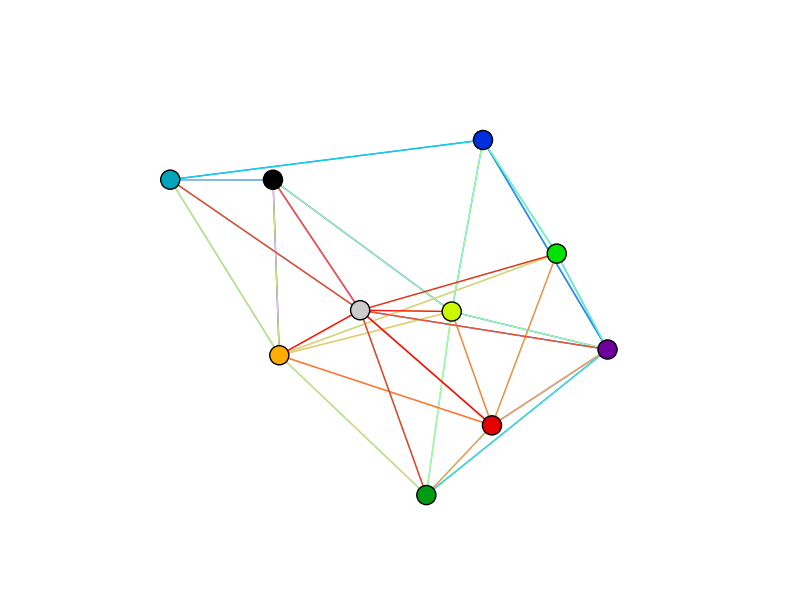
\includegraphics[width=0.45\columnwidth]{imagenes/exp1s10}
	\label{fig:grafo1s10}
}
\qquad
\subfigure[Grafo del experimento 1, para un tama\~no de 50 p\'aginas]{
	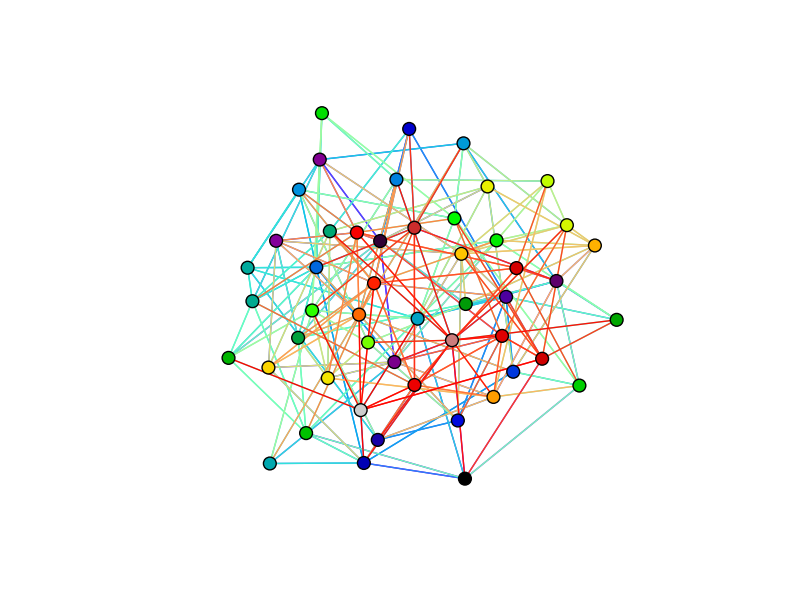
\includegraphics[width=0.45\columnwidth]{imagenes/exp1s50}
	\label{fig:grafo1s50}
}
\end{figure}

\begin{figure}[ht]
\subfigure[Grafo del experimento 1, para un tama\~no de 100 p\'aginas]{
	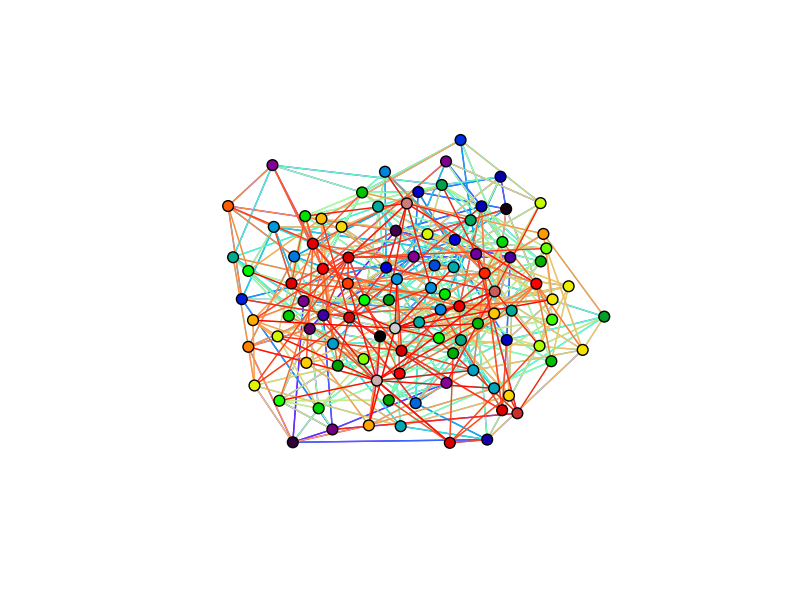
\includegraphics[width=0.45\columnwidth]{imagenes/exp1s100}
	\label{fig:grafo1s100}
}
\qquad
\subfigure[Grafo del experimento 1, para un tama\~no de 250 p\'aginas]{
	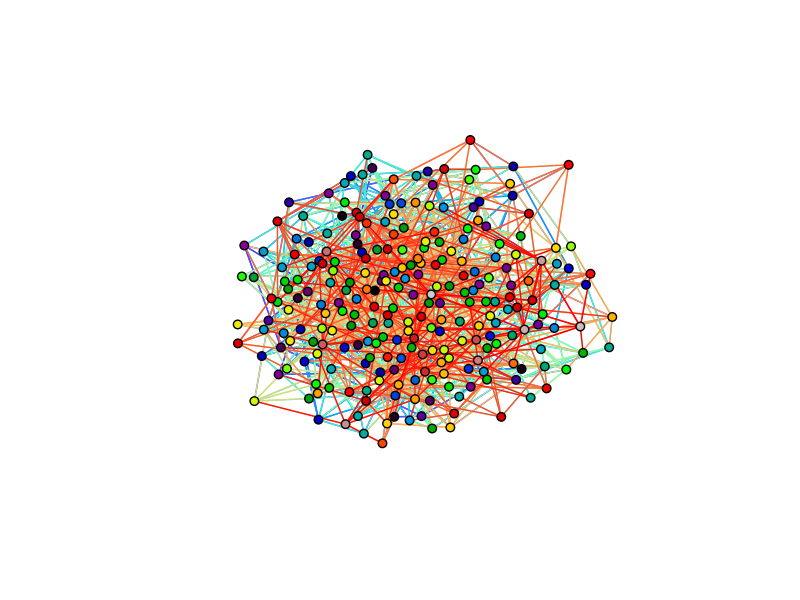
\includegraphics[width=0.45\columnwidth]{imagenes/exp1s250}
	\label{fig:grafo1s250}
}
\end{figure}


\FloatBarrier

\subsubsection{Experimento 2}
\par El experimento 2 es similar al primero: se observa c\'omo var\'ia el tiempo de ejecuci\'on al variar la cantidad de elementos no-nulos de la matriz de Markov.
La diferencia reside en modificar la cantidad de links que salen de cada p\'agina, manteniendo constante la cantidad total de p\'aginas -en particular, 1000 p\'aginas- 
(es decir, al rev\'es que en el experimento 1).
Si bien ambos experimentos miden lo mismo, el primero lo hace manteniendo de cierta forma la esparsidad de la matriz, mientras que el segundo lo hace modific\'andola.
En las figuras \ref{fig:grafo2s10}, \ref{fig:grafo2s50}, y \ref{fig:grafo2s100} se pueden ver graficados algunos de los inputs.
Cabe destacar como el grafo se vuelve paulatinamente m\'as interconectado.

\FloatBarrier

\begin{figure}[ht]
\subfigure[Grafo del experimento 2, para 1 link saliente por p\'agina]{
	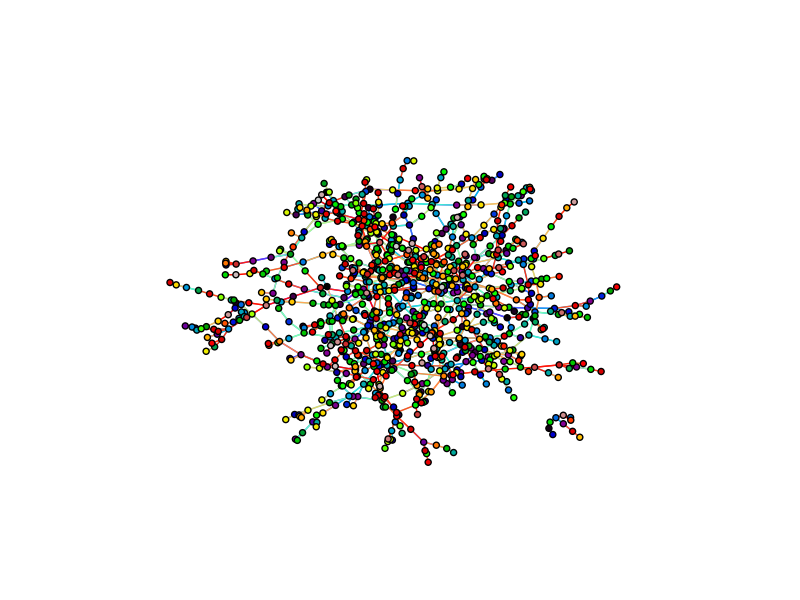
\includegraphics[width=0.45\columnwidth]{imagenes/exp2s10}
	\label{fig:grafo2s10}
}
\qquad
\subfigure[Grafo del experimento 2, para 2 links salientes por p\'agina]{
	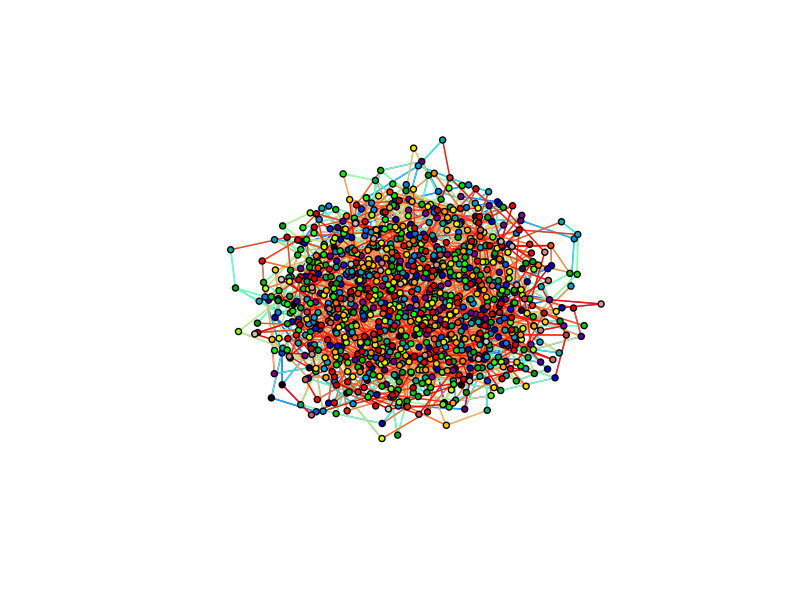
\includegraphics[width=0.45\columnwidth]{imagenes/exp2s50}
	\label{fig:grafo2s50}
}
\end{figure}

\begin{figure}[ht]
\subfigure[Grafo del experimento 2, para 4 links salientes por p\'agina]{
	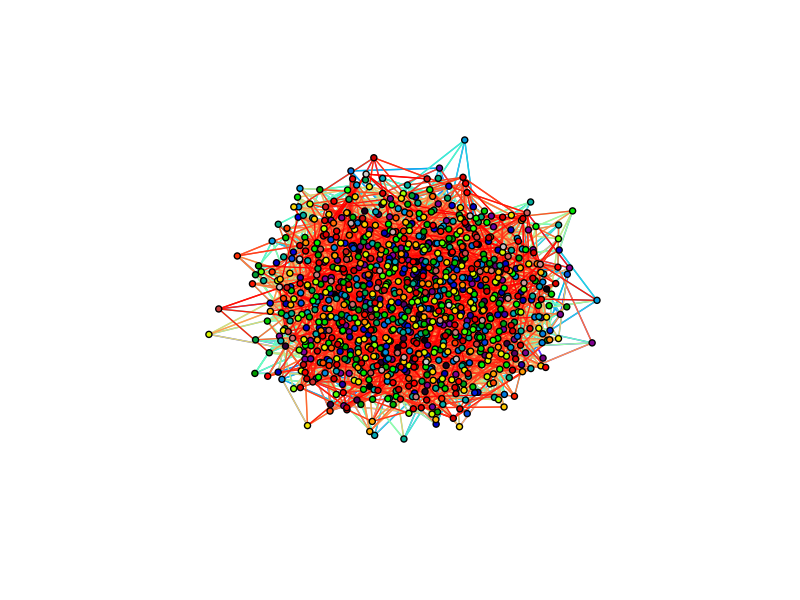
\includegraphics[width=0.45\columnwidth]{imagenes/exp2s100}
	\label{fig:grafo2s100}
}
\end{figure}


\FloatBarrier

\subsubsection{Resultados de los Experimentos 1 y 2}
\par En las figuras \ref{fig:res1}, y \ref{fig:res1zoom} se pueden observar los resultados del experimento 1 (la segunda figura muestra s\'olo los primeros 4 valores, por claridad).
En la figura \ref{fig:res2}, los del experimento 2.
Para permitirnos mejor comparar los resultados de ambos experimentos, se han incluido los dos juntos en la figura \ref{fig:res1y2} 
(la variable dependiente en este caso representa la cantidad de elementos no-nulos de la matriz).

\FloatBarrier
\begin{figure}[ht]
\begin{center}
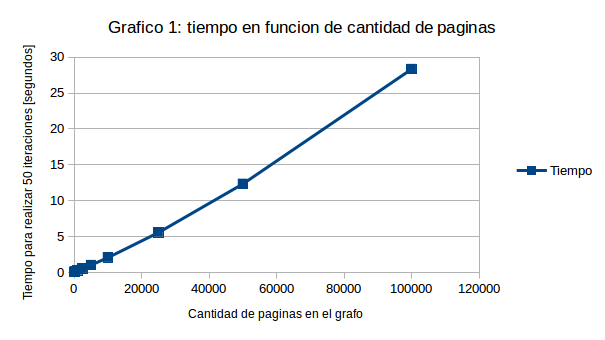
\includegraphics[width=0.8\columnwidth]{imagenes/graf1}
\caption{Resultado del experimento 1}
\label{fig:res1}
\end{center}
\end{figure}

\begin{figure}[ht]
\begin{center}
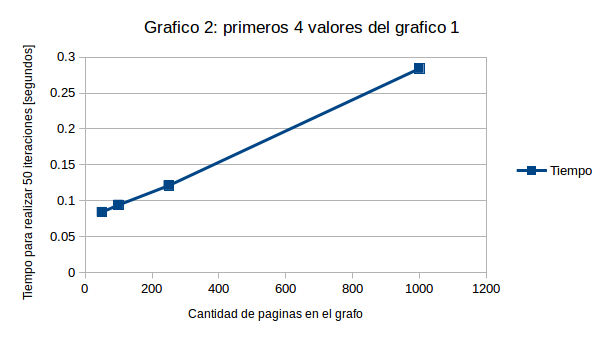
\includegraphics[width=0.8\columnwidth]{imagenes/graf2}
\caption{Resultado del experimento 1, primeros 4 valores}
\label{fig:res1zoom}
\end{center}
\end{figure}

\begin{figure}[ht]
\begin{center}
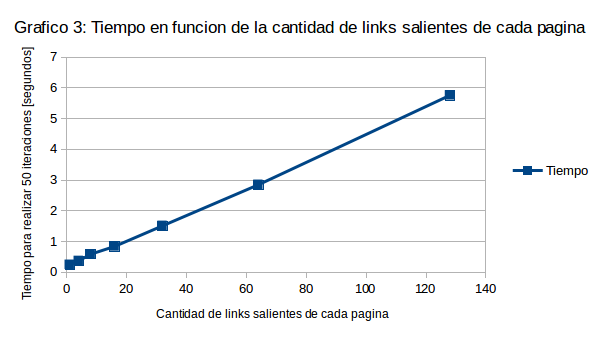
\includegraphics[width=0.8\columnwidth]{imagenes/graf3}
\caption{Resultado del experimento 2}
\label{fig:res2}
\end{center}
\end{figure}

\begin{figure}[ht]
\begin{center}
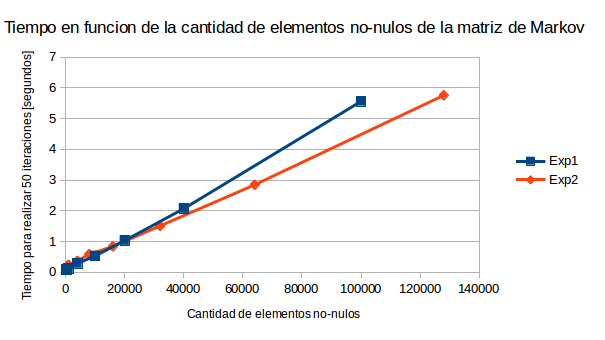
\includegraphics[width=0.8\columnwidth]{imagenes/graf6}
\caption{Resultado del experimento 1 y 2, juntos}
\label{fig:res1y2}
\end{center}
\end{figure}
\FloatBarrier

\par Se puede ver que los resultados de ambos experimentos describen curvas similares, pero la pendiente del primero es m\'as dr\'astica.
Esto es esperable, ya que si bien cada iteraci\'on del m\'etodo de la potencia depende linealmente de la cantidad de elementos no-nulos de la matriz,
tambi\'en depende linealmente de la cantidad de p\'aginas (el tama\~no de los vectores uniformes utilizados est\'a dado por la cantidad de nodos en el grafo, es decir de sitios en la red).

\subsubsection{Experimento 3}
\par Para el experimento 3, se medir\'a el tiempo de ejecuci\'on para una misma entrada (con 10000 p\'aginas y 4 links salientes de cada una), variando el par\'ametro \textit{''c''}.
\par Sabemos que \textit{''c''} es igual al módulo del segundo autovalor de la matriz
(como se encuentra demostrado en el paper \emph{The Second Eigenvalue of the Google Matrix}$^{\cite{Kamvar2}}$ de Kamvar y Haveliwala). Como vimos en la introducción teórica, el m\'etodo de la potencia trata obtener el primer autovalor al eliminar al resto en la combinaci\'on lineal, haciéndolos converger a 0 aplicando potenciación ya que son menores que 1. 
Cuanto mayor sea el $c$, y por ende, más cercano a 1 sea el módulo de $\lambda_2$, se espera que requiera de m\'as iteraciones para que $\lambda_2$ converja a 0 (en términos del algoritmo, que sea menor que $\varepsilon$).

\subsubsection{Experimento 4}
\par En el experimento 4, mediremos el tiempo de ejecuci\'on para la una misma entrada (id\'entica a la del tercer experimento) al variar el par\'ametro $\varepsilon$.

\subsubsection{Resultados de los Experimentos 3 y 4}
\par En las figuras \ref{fig:res3} y \ref{fig:res4} se encuentran los resultados de los experimentos 3 y 4, respectivamente.
Cabe destacar que la escala utilizada para el par\'ametro $\varepsilon$ en la figura \ref{fig:res4} es logar\'itmica.
\FloatBarrier

\begin{figure}[ht]
\begin{center}
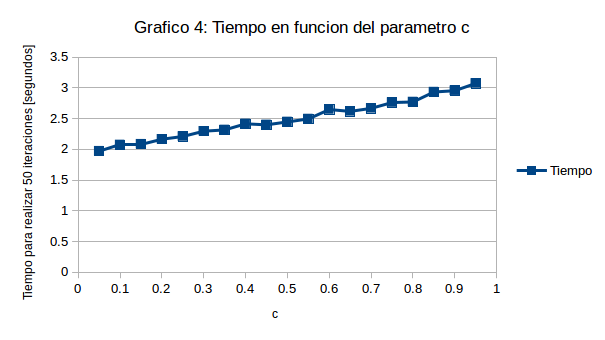
\includegraphics[width=0.8\columnwidth]{imagenes/graf4}
\caption{Resultado del experimento 3}
\label{fig:res3}
\end{center}
\end{figure}

\begin{figure}[ht]
\begin{center}
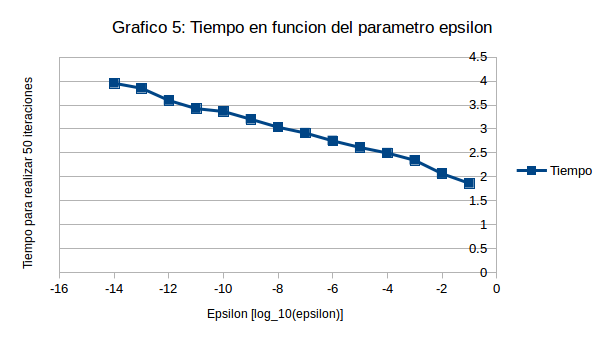
\includegraphics[width=0.8\columnwidth]{imagenes/graf5}
\caption{Resultado del experimento 4}
\label{fig:res4}
\end{center}
\end{figure}
\FloatBarrier

\par Se ve claramente que al aumentar el par\'ametro \textit{''c''} aumenta el tiempo de ejecución para computar el autovector principal. Lo mismo sucede al decrementar el $\varepsilon$, ya que disminuimos el margen que tomamos para traducir que los $|\lambda|$ convergen a 0.
\par Esto puede ser \'util si se desea realizar PageRank con un \textit{''c''} alto pero se debe calcular en un tiempo bajo, se puede incrementar $\varepsilon$ (aunque se pierda un poco de presici\'on).
\par Una observación es importante es que a pesar de que al disminuir el par\'ametro \textit{''c''} el algoritmo se vuelve más rápido, aumenta la probabilidad de teletransportación y esto puede dar lugar a páginas con un alto ranking injusto. (ver Experimento 3 de la sección de resultados para Competencias Deportivas).

\subsection{Experimentos sobre la eficacia de In-Deg, PageRank y PageRank con personalizaci\'on}
\subsubsection{Experimento 5}
\par El experimento 5 (y el 6) buscan comparar la eficiencia de PageRank e In-Deg en distintos escenarios.
Son dos de los ejemplos que m\'as comunmente se utilizan para detallar las ventajas de PageRank, y nuestra intenci\'on es comprobar que el algoritmo es efectivamente superior en estos casos.
\par En el caso del 5, la entrada consiste en un grafo donde hay una p\'agina ''central'' (como ser\'ian Google, Facebook, Wikipedia y dem\'as) a la que apunta la mayor\'ia de las p\'aginas.
El resto de las p\'aginas se distribuyen uniformemente (es decir, mediante una variable aleatoria uniforme) los links salientes.
La idea es que la p\'agina m\'as importante deber\'ia ser la central, y las que la siguen en prioridad deber\'ian ser p\'aginas apuntadas por \'esta.
En la figura \ref{fig:grafo5} se puede observar representado el input.

\FloatBarrier
\begin{figure}[ht]
\begin{center}
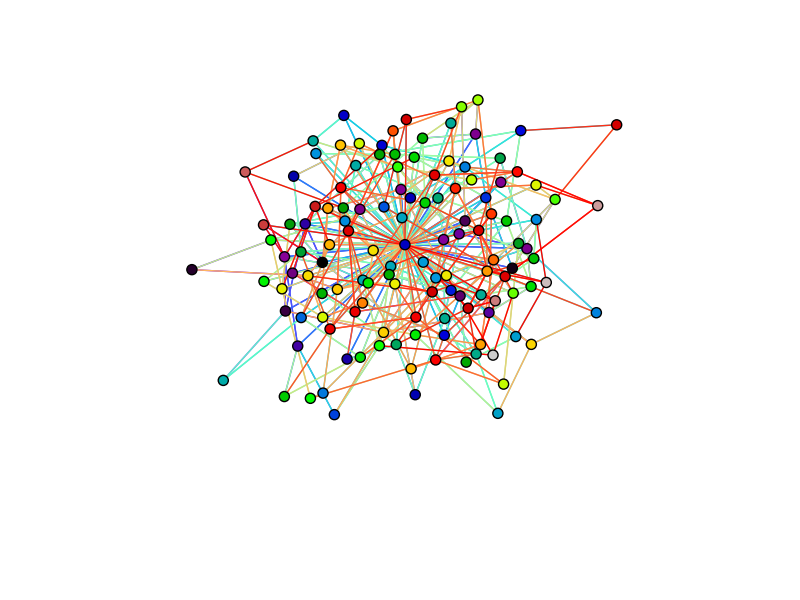
\includegraphics[width=0.8\columnwidth]{imagenes/exp5}
\caption{Grafo del experimento 5}
\label{fig:grafo5}
\end{center}
\end{figure}
\FloatBarrier

\subsubsection{Resultados del Experimento 5}
\par Tanto en In-Deg como en PageRank la p\'agina central es la primera en el ranking, pero en el caso de In-Deg la segunda es la p\'agina 36, que no es apuntada por la central.
En cambio en PageRank todas las primeras p\'aginas son apuntadas por la central, como es deseado.

\subsubsection{Experimento 6}
\par El experimento 6 consiste en juzgar la susceptibilidad de los m\'etodos a sucumbir bajo cierto tipo de ataque malicioso, donde una p\'agina crea otros sitios ''t\'iteres'' que apuntan a ella para aumentar su ranking.
Se espera que In-Deg sea m\'as vulnerable que PageRank, ya que estas p\'aginas maliciosas no son apuntadas por nadie 
(por lo que tienen un ranking inferior desde la perspectiva de PageRank, y por ende tendr\'an menor influencia en el orden final).
\par Se realizar\'an distintas iteraciones, manteniendo constante la cantidad de p\'aginas atacantes (en particular, 16 t\'iteres apuntando a un atacante), 
y variando la cantidad de p\'aginas normales, para ver como cambian los resultados al modificar la proporci\'on de p\'aginas atacantes y normales.
En las figuras \ref{fig:grafo6s64}, \ref{fig:grafo6s128} y \ref{fig:grafo6s256} se pueden observar los grafos que representan los distintos inputs.

\FloatBarrier
\begin{figure}[ht]
\subfigure[Grafo del experimento 6, para 64 p\'aginas normales]{
	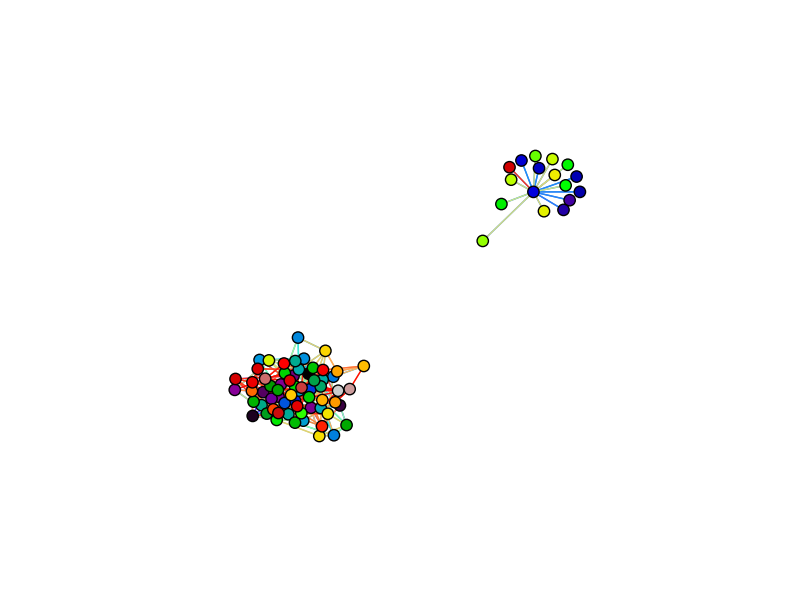
\includegraphics[width=0.45\columnwidth]{imagenes/exp6s64}
	\label{fig:grafo6s64}
}
\qquad
\subfigure[Grafo del experimento 6, para 128 p\'aginas normales]{
	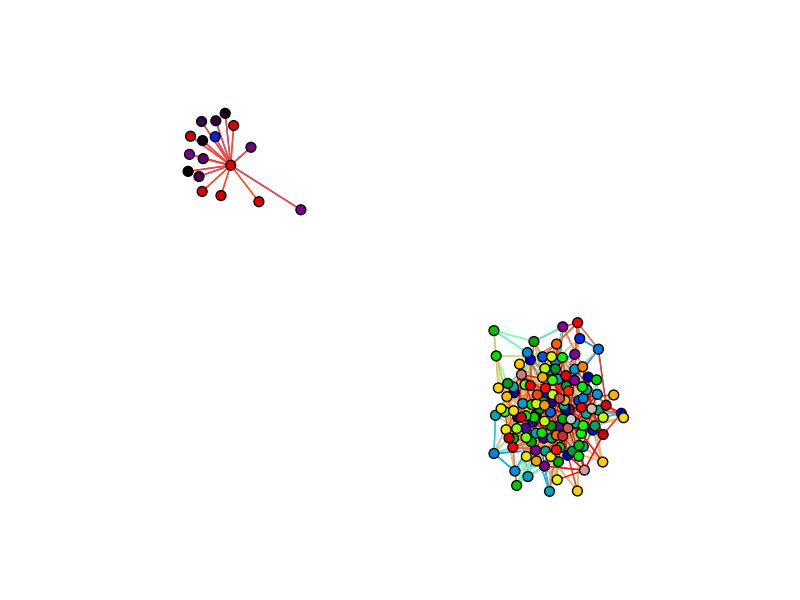
\includegraphics[width=0.45\columnwidth]{imagenes/exp6s128}
	\label{fig:grafo6s128}
}
\end{figure}

\begin{figure}[ht]
\subfigure[Grafo del experimento 6, para 256 p\'aginas normales]{
	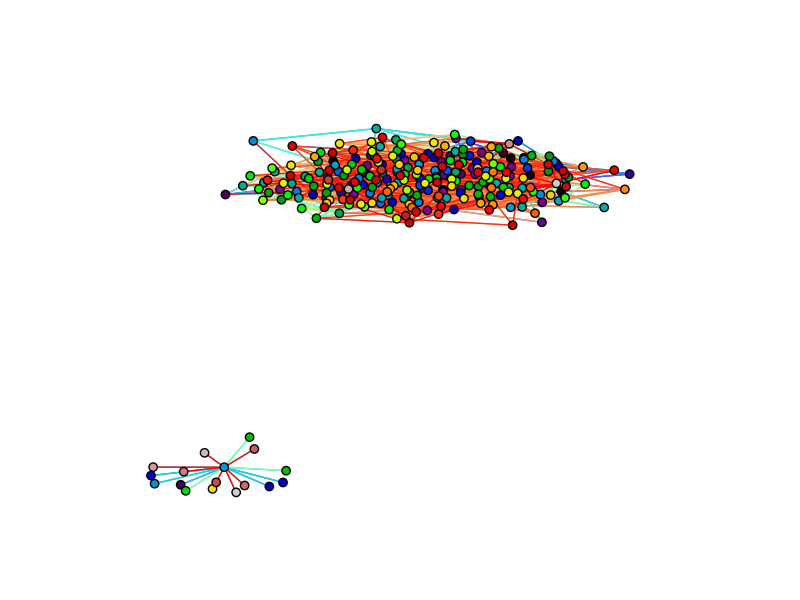
\includegraphics[width=0.45\columnwidth]{imagenes/exp6s256}
	\label{fig:grafo6s256}
}
\end{figure}

\FloatBarrier

\subsubsection{Resultados del Experimento 6}
\par En el caso de In-Deg, para las 3 entradas, la p\'agina atacante est\'a en la primera posici\'on del ranking.
En cambio, para PageRank, se encuentra en las posiciones 39, 77 y 153 (de un total de 81, 145 y 273, respectivamente).
Como se esperaba, PageRank es mucho menos vulnerable que In-Deg a este tipo de ataque.

\subsubsection{Experimento 7}
\par El s\'eptimo experimento busca juzgar la efectividad de nuestra variante de personalizaci\'on para el algoritmo PageRank.
Como entrada se utilizar\'a un grafo con 3 p\'aginas centrales (que se puede observar en la figura \ref{fig:grafo7}.
La idea es representar el resultado de un individuo buscando cierta expresi\'on en nuestro motor de b\'usqueda (por ejemplo ''Type of lambda expressions in C++11''),
y obteniendo como resultado ciertas p\'aginas, algunas de las cuales son ''centrales'' (como por ejemplo \textit{cplusplus.com}, \textit{cppreference.com} y \textit{stackoverflow.com})
y algunas son de menor importancia (por ejemplo blogs y otros sitios de ese tipo).
\par PageRank le asignar\'a un orden a estas p\'aginas, seguramente con las tres centrales arriba del ranking, pero cada usuario tendr\'a su propia preferencia de sitios.
Idealmente, el orden de los resultados de cada usuario tendr\'a en cuenta sus preferencias, y por ejemplo en el caso de las p\'aginas centrales, devolver\'a en primer lugar a su favorita.
Queremos comprobar que nuestro algoritmo de personalizaci\'on responde correctamente a un escenario de este tipo. 
Tambi\'en nos interesa ver como act\'ua frente a preferencias por sitios de menor importancia.
\par Realizaremos el mismo experimento con el mismo grafo de entrada previamente detallado, pero con diferentes entradas de personalizaci\'on.
En primer lugar, se utilizar\'a como control el resultado normal de PageRank; luego 3 historiales distintos donde el individuo prefiere cada una de las 3 p\'aginas centrales diferentes;
finalmente, un historial donde el usuario preferie mayoritariamente una p\'agina arbitraria.
Los historiales se encuentran detallados en los historiales 1, 2 y 3.
El par\'ametro \textit{''p''} de personalizaci\'on elegido es 0.5.

\FloatBarrier
\begin{figure}[ht]
\begin{center}
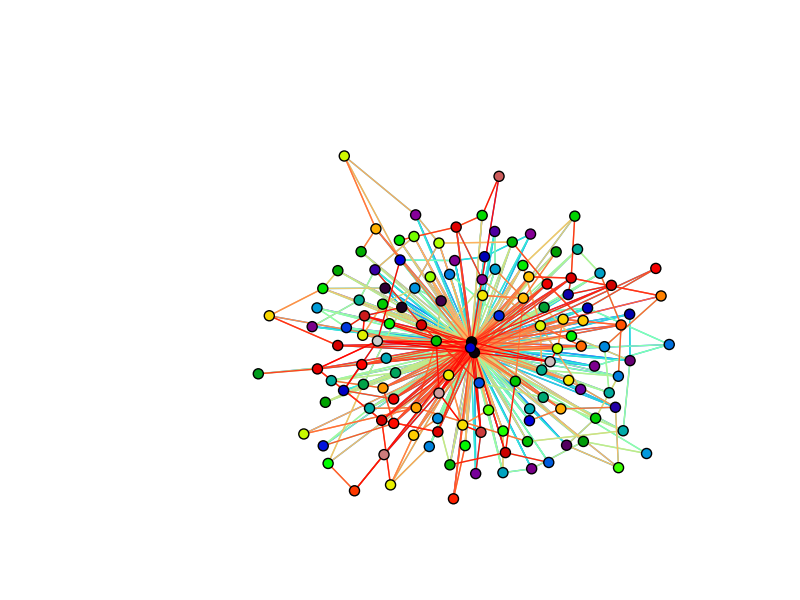
\includegraphics[width=0.8\columnwidth]{imagenes/exp7}
\caption{Grafo del experimento 7}
\label{fig:grafo7}
\end{center}
\end{figure}

\begin{multicols}{2}
\center
\begin{tabulary}{0.9\textwidth}{| c | c |}
\hline
\textbf{P\'agina} & \textbf{Cantidad de veces visitada} \\ \hline
5   & 19 \\ \hline
34  & 11 \\ \hline
80  & 12 \\ \hline
129 & 125\\ \hline
\end{tabulary}
\label{tab:in1}
Historial 1: Historial que prioritiza la p\'agina 129

\bigskip


\begin{tabulary}{0.9\textwidth}{| c | c |}
\hline
\textbf{P\'agina} & \textbf{Cantidad de veces visitada} \\ \hline
5   & 19 \\ \hline
34  & 11 \\ \hline
80  & 12 \\ \hline
130 & 125\\ \hline
\end{tabulary}
\label{tab:in2}
Historial 2: Historial que prioritiza la p\'agina 130

\bigskip


\begin{tabulary}{0.9\textwidth}{| c | c |}
\hline
\textbf{P\'agina} & \textbf{Cantidad de veces visitada} \\ \hline
5   & 19 \\ \hline
34  & 11 \\ \hline
80  & 12 \\ \hline
131 & 125\\ \hline
\end{tabulary}
\label{tab:in3}
Historial 3: Historial que prioritiza la p\'agina 131

\bigskip


\begin{tabulary}{0.9\textwidth}{| c | c |}
\hline
\textbf{P\'agina} & \textbf{Cantidad de veces visitada} \\ \hline
5   & 19 \\ \hline
34  & 11 \\ \hline
80  & 12 \\ \hline
124 & 125\\ \hline
\end{tabulary}
\label{tab:in4}
Historial 4: Historial que prioritiza la p\'agina 124

\bigskip

\end{multicols}

\subsubsection{Resultados del Experimento 7}


\begin{multicols}{2}
\center
\begin{tabulary}{0.9\textwidth}{| c | c |}
\hline
\textbf{Orden} & \textbf{P\'agina} \\ \hline
1   & 130\\ \hline
2   & 131\\ \hline
3   & 129\\ \hline
... & ---\\ \hline
46  & 5  \\ \hline
... & ---\\ \hline
67  & 124\\ \hline
\end{tabulary}
\label{tab:out1}
\linebreak
Tabla 1: Ranking de PageRank sin personalizaci\'on

\bigskip


\begin{tabulary}{0.9\textwidth}{| c | c |}
\hline
\textbf{Orden} & \textbf{P\'agina} \\ \hline
1   & 129\\ \hline
2   & 130\\ \hline
3   & 131\\ \hline
... & ---\\ \hline
9   & 5  \\ \hline
... & ---\\ \hline
\end{tabulary}
\label{tab:out2}
\linebreak
Tabla 2: Ranking de PageRank utilizando el historial que prioritiza la p\'agina 129

\bigskip


\begin{tabulary}{0.9\textwidth}{| c | c |}
\hline
\textbf{Orden} & \textbf{P\'agina} \\ \hline
1   & 130\\ \hline
2   & 131\\ \hline
3   & 129\\ \hline
... & ---\\ \hline
8   & 5  \\ \hline
... & ---\\ \hline
\end{tabulary}
\linebreak
Tabla 3: Ranking de PageRank utilizando el historial que prioritiza la p\'agina 130
\bigskip


\begin{tabulary}{0.9\textwidth}{| c | c |}
\hline
\textbf{Orden} & \textbf{P\'agina} \\ \hline
1   & 131\\ \hline
2   & 130\\ \hline
3   & 129\\ \hline
... & ---\\ \hline
15  & 5  \\ \hline
... & ---\\ \hline
\end{tabulary}
\label{tab:out4}
\linebreak
Tabla 4: Ranking de PageRank utilizando el historial que prioritiza la p\'agina 131

\columnbreak


\begin{tabulary}{0.9\textwidth}{| c | c |}
\hline
\textbf{Orden} & \textbf{P\'agina} \\ \hline
1   & 130\\ \hline
2   & 131\\ \hline
3   & 129\\ \hline
4   & 5  \\ \hline
... & ---\\ \hline
17  & 124\\ \hline
... & ---\\ \hline
\end{tabulary}
\label{tab:out5}
\linebreak
Tabla 5: Ranking de PageRank utilizando el historial que prioritiza la p\'agina 124, con $p = 0.5$

\bigskip


\begin{tabulary}{0.9\textwidth}{| c | c |}
\hline
\textbf{Orden} & \textbf{P\'agina} \\ \hline
1   & 5  \\ \hline
2   & 130\\ \hline
3   & 131\\ \hline
4   & 129\\ \hline
5   & 124\\ \hline
... & ---\\ \hline
\end{tabulary}
\label{tab:out6}
\linebreak
Tabla 6: Ranking de PageRank utilizando el historial que prioritiza la p\'agina 124, con $p = 0.95$

\bigskip


\begin{tabulary}{0.9\textwidth}{| c | c |}
\hline
\textbf{Orden} & \textbf{P\'agina} \\ \hline
1   & 130\\ \hline
2   & 131\\ \hline
3   & 129\\ \hline
4   & 5  \\ \hline
5   & 124\\ \hline
... & ---\\ \hline
\end{tabulary}
\label{tab:out7}
\linebreak
Tabla 7: Ranking de PageRank utilizando el historial que prioritiza la p\'agina 124, con $p = 0.75$ o $p = 0.85$

\bigskip

\end{multicols}

\par El resultado del control (que se puede observar en la tabla 1) efectivamente tiene a los 3 sitios centrales (en nuestro experimento, p\'aginas 129, 130 y 131) en las primeras 3 posiciones, en el orden 130, 131 y luego 129.
El sitio arbitrario (en este caso, el 124) se encuentra en el lugar 67 del ranking.
Las 3 iteraciones que prioritizan las distintas p\'aginas centrales (cuyos resultados se pueden encontrar en las tablas 2, 3 y 4) efectivamente tienen como resultado estos sitios en el primer lugar del ranking, que es lo deseado.
A su vez, la iteraci\'on (resultado en la tabla 5) que prioritiza la p\'agina arbitraria la tiene en el lugar 17.
Sin embargo, esta posici\'on es m\'as baja de la que esperamos debido a la alta prioridad que se le dio al sitio en el historial, 
lo que nos lleva a creer que \textit{''p''} en 0.5 puede ser demasiado sutil.
Realizamos nuevamente el experimento con \textit{''p''} en 0.85 y 0.95.
\par Con $p = 0.95$ (resultado en la tabla 6) la p\'agina 5 (que se encuentra en el historial de entrada, pero con frecuencia relativamente baja) sobrepasa a los sitios centrales.
Este resultado es excesivo, por lo que concluiremos que 0.95 es un valor demasiado alto para \textit{''p''}.
Tanto para $p = 0.85$ como para $p = 0.75$ (resultado en la tabla 7) la p\'agina 5 se encuentra en el cuarto lugar y la 124 en el quinto; por lo que concluimos que este es un rango aceptable para el par\'ametro de personalizaci\'on.

\newpage

\section{Resultados y Discusi\'on: Ligas Deportivas}
\par A continuaci\'on vamos a analizar resultados para el algoritmo GeM en el contexto de la Primera Divis\'on de la Liga Argentina de F\'utbol enfoc\'andonos en el ranking de equipos y experimentando sobre variaciones del ranking est\'andar, obtenci\'on del ranking mediante el m\'etodo GeM y m\'etodos alternatvos. Tomaremos como informaci\'on de entrada el campeonato 2015 hasta la fecha 26 inclusive. 
\bigskip

\par Contamos con el ranking oficial (est\'andar) de la liga que consta de ordenar los equipos por puntaje obtenido. Por cada partido ganado un equipo suma 3 puntos, por cada partido empatado obtiene tan solo 1, mientras que no obtiene puntos si fue derrotado. Como se puede ver el ranking no toma como informaci\'on relevante los goles. Mas adelante veremos que el m\'etodo GeM se basa fuertemente en los goles pero no diferencia entre victorias y derrotas tan notoriamente como si lo hace el ranking est\'andar.

\subsection{Experimento 1}
\par Como primer experimento vamos a comparar el ranking obtenido tras la aplicaci\'on del m\'etodo GeM y el ranking est\'andar tomando como entrada los resultados de todos los partidos hasta la fecha 26 inclusive. Creemos que van a notarse diferencias sobre todo por dos motivos:
\begin{itemize}
	\item El m\'etodo GeM no tiene en cuenta los empates, resultado que se da con frecuencia en el futbol argentino;
	\item El m\'etodo GeM solo se enfoca en los goles, mientras que el m\'etodo est\'andar solo se enfoca en quien gan\'o/empat\'o/perdi\'o.
\end{itemize}

\newpage

\subsubsection{Resultados del Experimento 1}

\begin{multicols}{2}
\center
\begin{tabulary}{0.45\textwidth}{| c | c | c | c | c |}
\hline
& \textbf{Equipo} & \textbf{Puntos} \\ \hline
1 & Boca Juniors & 58\\ \hline
2 & San Lorenzo & 54\\ \hline
3 & Rosario Central & 52\\ \hline
4 & Racing Club & 49\\ \hline
5 & River Plate & 48\\ \hline
6 & Independiente & 45\\ \hline
7 & Banfield & 43\\ \hline
8 & Belgrano & 43\\ \hline
9 & Estudiantes (LP) & 42\\ \hline
10 & Tigre & 42\\ \hline
11 & Quilmes & 39\\ \hline
12 & Lanús & 38\\ \hline
13 & Unión & 38\\ \hline
14 & Gimnasia y Esgrima (LP) & 37\\ \hline
15 & Newell's Old Boys & 33\\ \hline
16 & San Martín (SJ) & 32\\ \hline
17 & Aldosivi & 30\\ \hline
18 & Sarmiento & 30\\ \hline
19 & Argentinos Juniors & 29\\ \hline
20 & Olimpo & 29\\ \hline
21 & Temperley & 29\\ \hline
22 & Defensa y Justicia & 27\\ \hline
23 & Huracán & 26\\ \hline
24 & Vélez Sarsfield & 26\\ \hline
25 & Godoy Cruz & 25\\ \hline
26 & Colón & 24\\ \hline
27 & Arsenal & 23\\ \hline
28 & Atlético de Rafaela & 22\\ \hline
29 & Nueva Chicago & 17\\ \hline
30 & Crucero del Norte & 14\\ \hline
\end{tabulary}
\bigskip

Ranking mediante m\'etodo est\'andar.

\columnbreak

\begin{tabulary}{0.45\textwidth}{ | c | c | c |}
\hline
& \textbf{Equipo} & \textbf{Numero}\\ \hline
1 & Boca Juniors & 0.0860189\\ \hline
2 & Aldosivi & 0.0653536\\ \hline
3 & River Plate & 0.0634998\\ \hline
4 & San Lorenzo & 0.0620352\\ \hline
5 & Rosario Central & 0.0484731\\ \hline
6 & Racing Club & 0.0478783\\ \hline
7 & San Martín (SJ) & 0.0439558\\ \hline
8 & Quilmes & 0.0423821\\ \hline
9 & Newell's Old Boys & 0.0382332\\ \hline
10 & Vélez Sarsfield & 0.0376689\\ \hline
11 & Independiente & 0.0365646\\ \hline
12 & Belgrano & 0.0363978\\ \hline
13 & Gimnasia y Esgrima (LP) & 0.0335849\\ \hline
14 & Banfield & 0.0307372\\ \hline
15 & Estudiantes (LP) & 0.0295322\\ \hline
16 & Unión & 0.0288744\\ \hline
17 & Tigre & 0.0273356\\ \hline
18 & Sarmiento & 0.026108\\ \hline
19 & Huracán & 0.0246666\\ \hline
20 & Defensa y Justicia & 0.023737\\ \hline
21 & Lanús & 0.022729\\ \hline
22 & Olimpo & 0.0224689\\ \hline
23 & Arsenal & 0.0208702\\ \hline
24 & Godoy Cruz & 0.017516\\ \hline
25 & Temperley & 0.016045\\ \hline
26 & Crucero del Norte & 0.0160393\\ \hline
27 & Argentinos Juniors & 0.0153984\\ \hline
28 & Nueva Chicago & 0.0142318\\ \hline
29 & Atlético de Rafaela & 0.0113878\\ \hline
30 & Colón & 0.0102765\\ \hline
\end{tabulary}
\bigskip

Ranking mediante m\'etodo GeM.
\end{multicols}

\par En los resultados se puede observar que hay variaciones en las posiciones de los distintos equipos. Esto era de esperarse porque los m\'etodos usados se enfocan en distintos aspectos.
\bigskip

\par Vamos a analizar el caso particular de Aldosivi. En el ranking est\'andar se encuentra en la posici\'on 17, consecuencia de tan solo haber ganado 8 partidos y empatar 6 sobre 26 jugados. Mientras que en el ranking GeM se posiciona en el segundo lugar, veamos por qu\'e sucede esto. Recordemos que el m\'etodo GeM cuenta la diferencia de goles para con su rival en sus partidos ganados. Aldosivi, en los 8 partidos ganados no recibi\'o goles y convirti\'o 15. Cuenta entonces con una diferencia de goles importante, que lo posiciona en segundo lugar.

\par Con este claro ejemplo podemos ver la diferencia de enfoques de los dos m\'etodos. Creemos que para un deporte como el futbol el m\'etodo de GeM no est\'a bien formulado y no se enfoca en los resultados finales. Tal vez en otras ligas donde la diferencia de goles entre el ganador y el perdedor sea mayor (como la española o la alemana) y se den pocos empates pueda acercarse mas al m\'etodo est\'andar y/o competir con \'el sobre cu\'al deber\'ia ser el oficial.

\newpage

\subsection{Experimento 2}

\par Luego de analizar los resultados del experimento 1 queremos ver mas en detalle la influencia de los empates en el ranking obtenido por el m\'etodo GeM. Sabemos que al no tener en cuenta estos resultados nos alejamos del ranking est\'andar, pero queremos determinar si es factible que con alg\'un tipo de modificaci\'on podamos ajustarlo a un deporte con empates recurrentes (en este caso el f\'utbol).
\par Para tomar en consideraci\'on a los empates vamos a igualarlos a una victoria 1 a 0: ``empate = victoria por 1 a 0''. Sabemos que \'esto influye positivamente sobre los equipos con muchos empates, pero al darle un resultado favorable m\'inimo (1 a 0) creemos que no afectar\'a demasiado, manteniendo as\'i la base del enfoque del m\'etodo GeM y d\'andole cierta importancia a los empates.

\subsubsection{Resultados del Experimento 2}

\begin{figure}[ht]
\begin{center}
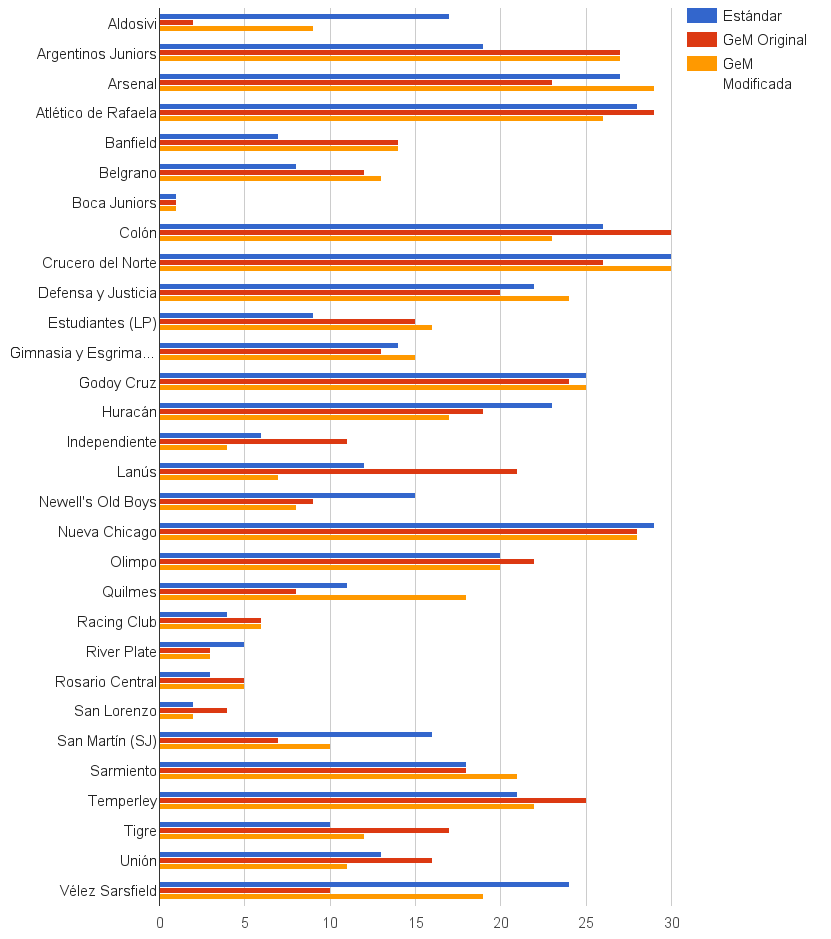
\includegraphics[width=0.7\columnwidth]{../src/experimentos/deportivos/2/experimento2.png}
\caption{Comparaciones de Rankings}
\end{center}
\end{figure}

\par En los resultados obtenidos vemos que la modificaci\'on del m\'etodo GeM gener\'o cambios en el posicionamiento de los equipos con empates en su historial. En algunos casos estos cambios lo alejaron de su posicionamiento en el ranking est\'andar mientras que en la mayor\'ia de los casos lo acercaron, d\'andole as\'i un cierto valor al empate que antes no era tenido en cuenta. Como nombramos antes, mantuvimos el enfoque del m\'etodo GeM pero le agregamos un pequeño valor a los empates que los gener\'o una tabla que creemos mas adecuada a la realidad del f\'utbol.

\newpage

\begin{multicols}{2}
\center
\begin{tabulary}{0.45\textwidth}{| c | c | c | c | c |}
\hline
& \textbf{Equipo} & \textbf{Puntos} \\ \hline
1 & Boca Juniors & 58\\ \hline
2 & San Lorenzo & 54\\ \hline
3 & Rosario Central & 52\\ \hline
4 & Racing Club & 49\\ \hline
5 & River Plate & 48\\ \hline
6 & Independiente & 45\\ \hline
7 & Banfield & 43\\ \hline
8 & Belgrano & 43\\ \hline
9 & Estudiantes (LP) & 42\\ \hline
10 & Tigre & 42\\ \hline
11 & Quilmes & 39\\ \hline
12 & Lanús & 38\\ \hline
13 & Unión & 38\\ \hline
14 & Gimnasia y Esgrima (LP) & 37\\ \hline
15 & Newell's Old Boys & 33\\ \hline
16 & San Martín (SJ) & 32\\ \hline
17 & Aldosivi & 30\\ \hline
18 & Sarmiento & 30\\ \hline
19 & Argentinos Juniors & 29\\ \hline
20 & Olimpo & 29\\ \hline
21 & Temperley & 29\\ \hline
22 & Defensa y Justicia & 27\\ \hline
23 & Huracán & 26\\ \hline
24 & Vélez Sarsfield & 26\\ \hline
25 & Godoy Cruz & 25\\ \hline
26 & Colón & 24\\ \hline
27 & Arsenal & 23\\ \hline
28 & Atlético de Rafaela & 22\\ \hline
29 & Nueva Chicago & 17\\ \hline
30 & Crucero del Norte & 14\\ \hline
\end{tabulary}
\bigskip

Ranking mediante m\'etodo est\'andar.

\columnbreak

\begin{tabulary}{0.4\textwidth}{ | c | c | c |}
\hline
& \textbf{Equipo} & \textbf{Numero}\\ \hline
1 & Boca Juniors & 0.0532173\\ \hline
2 & San Lorenzo & 0.0466695\\ \hline
3 & River Plate & 0.0466113\\ \hline
4 & Independiente & 0.0443246\\ \hline
5 & Rosario Central & 0.0436734\\ \hline
6 & Racing Club & 0.0391814\\ \hline
7 & Lanús & 0.0385408\\ \hline
8 & Newell's Old Boys & 0.0383858\\ \hline
9 & Aldosivi & 0.0381275\\ \hline
10 & San Martín (SJ) & 0.0370988\\ \hline
11 & Unión & 0.0370056\\ \hline
12 & Tigre & 0.0347199\\ \hline
13 & Belgrano & 0.0340198\\ \hline
14 & Banfield & 0.0340106\\ \hline
15 & Gimnasia y Esgrima (LP) & 0.0326107\\ \hline
16 & Estudiantes (LP) & 0.0319726\\ \hline
17 & Huracán & 0.0312592\\ \hline
18 & Quilmes & 0.0308084\\ \hline
19 & Vélez Sarsfield & 0.0306859\\ \hline
20 & Olimpo & 0.0304997\\ \hline
21 & Sarmiento & 0.0302557\\ \hline
22 & Temperley & 0.0277299\\ \hline
23 & Colón & 0.0267565\\ \hline
24 & Defensa y Justicia & 0.0262358\\ \hline
25 & Godoy Cruz & 0.024695\\ \hline
26 & Atlético de Rafaela & 0.024516\\ \hline
27 & Argentinos Juniors & 0.023696\\ \hline
28 & Nueva Chicago & 0.023149\\ \hline
29 & Arsenal & 0.0230411\\ \hline
30 & Crucero del Norte & 0.0165022\\ \hline
\end{tabulary}
\bigskip

Ranking obtenido por el m\'etodo GeM modificado.
\end{multicols}

\par Haciendo referencia al experimento 1, donde supimos comparar el ranking est\'andar del obtenido por el m\'etodo GeM, podemos sumar los resultados obtenidos con el m\'etodo GeM modificado. Notamos que las similitudes son mayores  a pesar de mantener distancia en los enfoques.

\newpage

\subsection{Experimento 3}

\par En este experimento analizaremos el impacto de la variación del parámetro $c$ sobre los resultados de rankings de competencias deportivas usando GeM. Vimos, por resultados anteriores, que aumentar el $c$ hace que el algoritmo se vuelva más lento, ya que tarda más en converger, pero devuelve resultados más justos. En este experimento nos centraremos en las diferencias entre los resultados y no en el tiempo de ejecución (ver Experimento 3 de la sección de resultados para Páginas Web).

\par Para llevar a cabo el experimento compararemos las tablas de posiciones obtenidas por cada equipo para ciertos valores de $c$, comparándolas con la posición actual en el ranking de la AFA.

\subsubsection{Resultados del Experimento 3}

\par Observemos la comparación entre las posiciones obtenidas por los equipos según cada $c$:

\begin{tabulary}{\textwidth}{| c | c | c | c | c | c | c |}
\hline						
\textbf{Pos. AFA} & \textbf{Equipo} & \textbf{c=0.85} & \textbf{c=0.65} & \textbf{c=0.45} & \textbf{c=0.25} & \textbf{c=0.00}\\ \hline
1 & Boca Juniors & 1 & 1 & 1 & 1 & 1 \\ \hline
2 & San Lorenzo & 4 & 3 & 2 & 2 & 1\\ \hline
3 & Rosario Central & 5 & 6 & 6 & 5 & 1\\ \hline
4 & Racing Club & 6 & 5 & 5 & 4 & 1\\ \hline
5 & River Plate & 3 & 2 & 3 & 3 & 1\\ \hline
6 & Independiente & 11 & 9 & 9 & 8 & 1\\ \hline
7 & Banfield & 14 & 14 & 13 & 13 & 1\\ \hline
8 & Belgrano & 12 & 11 & 10 & 9 & 1\\ \hline
9 & Estudiantes (LP) & 15 & 15 & 16 & 16 & 1\\ \hline
10 & Tigre & 17 & 15 & 15 & 14 & 1\\ \hline
11 & Quilmes & 8 & 7 & 7 & 7 & 1\\ \hline
12 & Lanús & 21 & 19 & 18 & 14 & 1\\ \hline
13 & Unión & 16 & 16 & 17 & 18 & 1\\ \hline
14 & Gimnasia y Esgrima (LP) & 13 & 13 & 12 & 12 & 1\\ \hline
15 & Newell's Old Boys & 9 & 10 & 11 & 11 & 1\\ \hline
16 & San Martín (SJ) & 7 & 8 & 8 & 10 & 1\\ \hline
17 & Aldosivi & 2 & 4 & 4 & 6 & 1\\ \hline
18 & Sarmiento & 18 & 18 & 19 & 19 & 1\\ \hline
19 & Argentinos Juniors & 27 & 26 & 25 & 25 & 1\\ \hline
20 & Olimpo & 22 & 23 & 23 & 23 & 1\\ \hline
21 & Temperley & 25 & 25 & 26 & 26 & 1\\ \hline
22 & Defensa y Justicia & 20 & 21 & 22 & 22 & 1\\ \hline
23 & Huracán & 19 & 20 & 20 & 20 & 1\\ \hline
24 & Vélez Sarsfield & 10 & 12 & 14 & 17 & 1\\ \hline
25 & Godoy Cruz & 24 & 24  & 24 & 24 & 1\\ \hline
26 & Colón & 30 & 30 & 30 & 30 & 1\\ \hline
27 & Arsenal & 23 & 22 & 21 & 21 & 1\\ \hline
28 & Atlético de Rafaela & 29 & 29 & 29 & 29 & 1\\ \hline
29 & Nueva Chicago & 28 & 28 & 28 & 28 & 1\\ \hline
30 & Crucero del Norte & 26 & 27 & 27 & 27 & 1\\ \hline
\end{tabulary}

\hspace{1cm}

\par Para las fechas del torneo de la AFA, no se ven grandes cambios en los resultados obtenidos variando el $c$ excepto en los casos de Lanús, y Vélez. Esto es una diferencia con el contexto de Páginas Web, ya que como las matrices de Markov de las competencias de fútbol no son esparsas (todos juegan contra todos), a diferencia del caso de las páginas web, no se nota tanto el impacto de la teletransportación. Sin embargo, como vimos en experimentos anteriores, debido a las diferencias de modelado del empate no podemos comparar cualitativamente si los resultados son más justos. 
\par Además, podemos ver que al disminuir el $c$ las distribuciones del vector estacionario se vuelven más equitativas, siendo el caso extremo $c = 0$, donde como se ve en la tabla, todos los equipos terminan en la misma posición.



 
\newpage

\section{Conclusiones}

\par Concluimos que el algoritmo PageRank es superior al In-Deg para establecer un ranking de p\'aginas web.
Tambi\'en concluimos que el tiempo de convergencia depende no s\'olo de la cantidad de elementos no-nulos de la matriz de transici\'on (es decir, la cantidad de v\'ertices en el grafo que representa a la red), sino de la cantidad de p\'aginas en la web representada (la cantidad de nodos en el grafo).
Adicionalmente, concluimos que el tiempo de convergencia aumenta al incrementar el par\'ametro \textit{''c''}.
\par Tambi\'en concluimos que nuestra variante del algoritmo PageRank de personalizaci\'on es efectiva, cuando se emplea un par\'ametro \textit{``p''} apropiado (alrededor del rango [0.75, 0.85].

\bigskip

\par Por parte de la aplicaci\'on del m\'etodo GeM en ligas deportivas podemos concluir que es un m\'etodo interesante para realizar comparaciones con los rankings est\'andar. Nos deja con ganas de experimentar sobre otras ligas o deportes y ver que resultados obtenemos. Por cuestiones de tiempo no pudimos llevar a cabo estos experimentos, pero sabemos que podemos ir ajustando los par\'ametros y variando algunos pasos del m\'etodo para lograr resultados diversos y enfocar el ranking en los datos que creamos importantes.
\par Pudimos notar que los tiempos de ejecuci\'on no fueron relevantes y no tuvimos necesidad de optimizar el proceso ni las estructuras de memoria, dado que los datos eran muy acotados.
\par 

\bigskip

\par En terminos generales pudimos tomar m\'etodos num\'ericos y aplicarlos sobre casos reales. Esto implic\'o tener cuidado con los costos (tanto de tiempo como de memoria) y verificar los resultados con respecto a los datos reales. No nos llevamos grandes sorpresas pero nos pareci\'o interesante y entretenido poder aplicar el TP a casos reales y cercanos a la vida diaria y ver como se comportaban.
 
\newpage

\section{Ap\'endices}

\subsection{Apéndice A}


\vskip 5pt
\noindent\textbf{Enunciado}
\vskip 5pt

El objetivo del trabajo es experimentar en el contexto planteado utilizando el algoritmo PageRank con las variantes propuestas. A su vez, se busca
comparar los resultados obtenidos cualitativa y cuantitativamente con los algoritmos tradicionales utilizados en cada uno de los contextos planteados. 
Los m\'etodos a implementar (como m\'inimo) en ambos contexto planteados por el trabajo son los siguientes:

\begin{enumerate}
\item \emph{B\'usqueda de p\'aginas web:} PageRank e \textsc{In-deg}, \'este \'ultimo consiste en definir el ranking de las p\'aginas utilizando 
solamente la cantidad de ejes entrantes a cada una de ellas, orden\'andolos en forma decreciente.
\item \emph{Rankings en competencias deportivas:} GeM y al menos un m\'etodo est\'andar propuesto por el grupo (ordenar por victorias/derrotas,
puntaje por ganado/empatado/perdido, etc.) en funci\'on del deporte(s) considerado(s).
\end{enumerate}

El contexto considerado en 1., en la b\'usqueda de p\'aginas web, representa un desaf\'io no s\'olo desde el modelado, si no tambi\'en desde el punto 
de vista computacional considerando la dimensi\'on de la informaci\'on y los datos a procesar. Luego, dentro de nuestras posibilidades, consideramos
un entorno que simule el contexto real de aplicaci\'on donde se abordan  instancias de gran escala (es decir, $n$, el n\'umero total de p\'aginas, es 
grande). Para el desarrollo de PageRank, se pide entonces considerar el trabajo de Bryan y Leise \cite{Bryan2006} donde se explica la intuci\'on y algunos 
detalles t\'ecnicos respecto a PageRank. Adem\'as, en Kamvar et al. \cite{Kamvar2003} se propone una mejora del mismo. Si bien esta mejora queda fuera de 
los alcances del trabajo, en la Secci\'on 1 se presenta una buena formulaci\'on del algoritmo. En base a su definici\'on, $P_2$ no es una matriz esparsa. 
Sin embargo, en Kamvar et al. \cite[Algoritmo 1]{Kamvar2003} se propone una forma alternativa para computar $x^{(k+1)} = P_2 x^{(k)}$. Este resultado debe 
ser utilizado para mejorar el almacenamiento de los datos.

En la pr\'actica, el grafo que representa la red de p\'aginas suele ser esparso, es decir, una p\'agina posee relativamente pocos links de salida comparada 
con el n\'umero total de p\'aginas. A su vez, dado que $n$ tiende a ser un n\'umero muy grande, es importante tener en cuenta este hecho a la hora de definir 
las estructuras de datos a utilizar. Luego, desde el punto de vista de implementaci\'on se pide utilizar alguna de las siguientes estructuras de datos para 
la representaci\'on de las matrices esparsas: \emph{Dictionary of Keys} (dok), \emph{Compressed Sparse Row} (CSR) o \emph{Compressed Sparse Column} (CSC). 
Se deber\'a incluir una justificaci\'on respecto a la elecci\'on que consdiere el contexto de aplicaci\'on. Adem\'as, para PageRank se debe implementar el 
m\'etodo de la potencia para calcular el autovector principal. Esta implementaci\'on debe ser realizada \'integramente en \textsc{C++}.

En funci\'on de la experimentaci\'on, se deber\'a realizar un estudio particular para cada algoritmo (tanto en t\'erminos de comportamiento
del mismo, como una evaluaci\'on de los resultados obtenidos) y luego se proceder\'a a comparar cualitativamente los rankings generados.
La experimentaci\'on deber\'a incluir como m\'inimo los siguientes experimentos:
\begin{enumerate}
\item Estudiar la convergencia de PageRank, analizando la evoluci\'on de la norma Manhattan (norma $L_1$) entre dos iteraciones sucesivas. Comparar los 
resultados obtenidos para al menos dos instancias de tama\~no mediano-grande, variando el valor de $c$. 
\item Estudiar el tiempo de c\'omputo requerido por PageRank. 
\item Para cada algoritmo, proponer ejemplos de tama\~no peque\~no que ilustren el comportamiento esperado (puede ser utilizando las herramientas provistas
por la c\'atedra o bien generadas por el grupo).
\end{enumerate}

Puntos opcionales:
\begin{enumerate}
\item Demostrar que los pasos del Algoritmo 1 propuesto en Kamvar et al. \cite{Kamvar2003} son correctos y computan $P_2 x$.
\item Establecer una relaci\'on con la proporci\'on entre $\lambda_1 = 1$ y $|\lambda_2|$ para la convergencia de PageRank.
\end{enumerate}

El segundo contexto de aplicaci\'on no presenta mayores desaf\'ios desde la perspectiva computacional, ya que en el peor de los casos una liga no suele tener
mas que unas pocas decenas de equipos. M\'as a\'un, es de esperar que en general la matriz que se obtiene no sea esparsa, ya que probablemente un equipo juegue
contra un n\'umero significativo de contrincantes. Sin embargo, la popularidad y sensibilidad del problema planteado requieren de un estudio detallado y 
pormenorizado de la calidad de los resultados obtenidos. El objetivo en este segundo caso de estudio es puramente experimental. 

En funci\'on de la implementaci\'on, a\'un cuando no represente la mejor opci\'on, es posible reutilizar y adaptar el desarrollo realizado para p\'aginas web. 
Tambi\'en es posible realizar una nueva implementaci\'on desde cero, simplificando la operatoria y las estructuras, en \textsc{C++}, \textsc{Matlab} o 
\textsc{Python}.

La experimentaci\'on debe ser realizada con cuidado, analizando (y, eventualmente, modificando) el modelo de GeM:
\begin{enumerate}
\item Considerar al menos un conjunto de datos reales, con los resultados de cada fecha para alguna liga de algu\'un deporte.
\item Notar que el m\'etodo GeM asume que no se producen empates entre los equipos (o que si se producen, son poco frecuentes). En caso de considerar un 
deporte donde el empate se da con cierta frecuencia no despreciable (por ejemplo, f\'utbol), es fundamental aclarar como se refleja esto en el modelo y 
analizar su eventual impacto.
\item Realizar experimentos variando el par\'ametro $c$, indicando como impacta en los resultados. Analizar la evoluci\'on del ranking de los equipos a 
trav\'es del tiempo, evaluando tambi\'en la evoluci\'on de los rankings e identificar caracter\'isticas/hechos particulares que puedan ser determinantes 
para el modelo, si es que existe alguno.
\item Comparar los resultados obtenidos con los reales de la liga utilizando el sistema est\'andar para la misma.
\end{enumerate}

Puntos opcionales:
\begin{enumerate}
\item Proponer (al menos) dos formas alternativas de modelar el empate entre equipos en GeM.
\end{enumerate}


\vskip 5pt
\noindent\textbf{Par\'ametros y formato de archivos}
\vskip 5pt

El programa deber\'a tomar por l\'inea de comandos dos par\'ametros. El primero de ellos contendr\'a la informaci\'on del experimento, incluyendo
el m\'etodo a ejecutar (\verb+alg+, 0 para PageRank, 1 para el m\'etodo alternativo), la probabilidad de teletransportaci\'on $c$, el tipo de instancia
(0 p\'aginas web, 1 deportes), el \emph{path} al archivo/directorio conteniendo la definici\'on de la red (que debe ser relativa al ejecutable, o el path 
absoluto al archivo) y el valor de tolerancia utilizado en el criterio de parada del m\'etodo de la potencia. 

El siguiente ejemplo muestra un caso donde se pide ejecutar PageRank, con una probabilidad de teletransportaci\'on de 0.85, sobre la red descripta en 
\verb+test1.txt+ (que se encuentra en el directorio \verb+tests/+), correspondiente a una instancia de ranking aplicado a deportes y con una tolerancia 
de corte de $0.0001$.
\begin{verbatim}
0 0.85 1 tests/red-1.txt 0.0001
\end{verbatim}

Para la definici\'on del grafo que representa la red, se consideran dos bases de datos de instancias con sus correspondientes formatos. La primera
de ellas es el conjunto provisto en SNAP \cite{SNAP} (el tipo de instancia es 0), con redes de tama\~no grande obtenidos a partir de datos reales. Adem\'as, 
se consideran las instancias que se forman a partir de resultados de partidos entre equipos, para alg\'un deporte elegido por el grupo. 

En el caso de la base de SNAP, los archivos contiene primero cuatro l\'ineas con informaci\'on sobre la instancia (entre ellas, $n$ y la cantidad
total de links, $m$) y luego $m$ l\'ineas con los pares $i$, $j$ indicando que $i$ apunta a $j$. A modo de ejemplo, a continuaci\'on se muestra el 
archivo de entrada correspondiente a la red propuesta en Bryan y Leise \cite[Figura 1]{Bryan2006}: 

\begin{verbatim}
# Directed graph (each unordered pair of nodes is saved once): 
# Example shown in Bryan and Leise.
# Nodes: 4 Edges: 8 
# FromNodeId    ToNodeId
1   2
1   3
1   4
2   3
2   4
3   1
4   1
4   3
\end{verbatim}

Para el caso de rankings en ligas deportivas, el archivo contiene primero una l\'inea con informaci\'on sobre la cantidad de equipos ($n$), y la cantidad
de partidos totales a considerar ($k$). Luego, siguen $k$ l\'neas donde cada una de ellas representa un partido y contiene la siguiente informaci\'on: 
n\'umero de fecha (es un dato opcional al problema, pero que puede ayudar a la hora de experimentar), equipo $i$, goles equipo $i$, equipo $j$, goles equipo $j$.
A continuaci\'on se muestra el archivo de entrada con la informaci\'on del ejemplo utilizado en Govan et al. \cite{Govan2008}:

\begin{verbatim}
6 10
1 1 16 4 13
1 2 38 5 17
1 2 28 6 23
1 3 34 1 21
1 3 23 4 10
1 4 31 1 6
1 5 33 6 25
1 5 38 4 23
1 6 27 2 6
1 6 20 5 12
\end{verbatim}

Es importante destacar que, en este \'ultimo caso, los equipos son identificados mediante un n\'umero. Opcionalmente podr\'a considerarse un archivo que contenga, 
para cada equipo, cu\'al es el c\'odigo con el que se lo identifica.

Una vez ejecutado el algoritmo, el programa deber\'a generar un archivo de salida que contenga una l\'inea por cada
p\'agina ($n$ l\'ineas en total), acompa\~nada del puntaje obtenido por el algoritmo PageRank/\textsc{In-deg}/m\'etodo alternativo. 

Para generar instancias de p\'aginas web, es posible utilizar el c\'odigo Python provisto por la c\'atedra. La utilizaci\'on del mismo se
encuentra descripta en el archivo README. Es importante mencionar que, para que el mismo funcione, es
necesario tener acceso a Internet. En caso de encontrar un bug en el mismo, por favor contactar a los docentes de la
materia a trav\'es de la lista. Desde ya, el c\'odigo puede ser modificado por los respectivos grupos agregando todas
aquellas funcionalidades que consideren necesarias.

Para instancias correspondientes a resultados entre equipos, la c\'atedra provee un conjunto de archivos con los resultados del Torneo de Primera Divisi\'on 
del F\'utbol Argentino hasta la Fecha 23. Es importante aclarar que los dos partidos suspendidos, River - Defensa y Justicia y Racing - Godoy Cruz han sido 
arbitrariamente completados con un resultado inventado, para simplificar la instancia. En funci\'on de datos reales, una alternativa es considerar el 
repositorio DataHub \cite{datahub}, que contiene informaci\'on estad\'istica y resultados para distintas ligas y deportes de todo el mundo.

\vskip 5pt

%\subsection{Apéndice B}
%
%\textbf{Código fuente para ...}
%\textbf{}

%\lstset{language=C++, breaklines=true, basicstyle=\footnotesize}
%\begin{lstlisting}[frame=single]
%
%\end{lstlisting}

 
\newpage

\section{Referencias}

\begin{thebibliography}{1}

\bibitem{datahub}
Datahub.
\newblock \url{http://datahub.io}.

\bibitem{SNAP}
Stanford large network dataset collection.
\newblock \url{http://snap.stanford.edu/data/#web}.

\bibitem{Brin1998}
Sergey Brin and Lawrence Page.
\newblock {The anatomy of a large-scale hypertextual Web search engine}.
\newblock {\em Computer Networks and ISDN Systems}, 30(1-7):107--117, April
  1998.

\bibitem{Bryan2006}
Kurt Bryan and Tanya Leise.
\newblock The linear algebra behind google.
\newblock {\em SIAM Review}, 48(3):569--581, 2006.

\bibitem{Govan2008}
Angela~Y. Govan, Carl~D. Meyer, and Rusell Albright.
\newblock Generalizing google's pagerank to rank national football league
  teams.
\newblock In {\em Proceedings of SAS Global Forum 2008}, 2008.

\bibitem{Kamvar2003}
Sepandar~D. Kamvar, Taher~H. Haveliwala, Christopher~D. Manning, and Gene~H.
  Golub.
\newblock Extrapolation methods for accelerating pagerank computations.
\newblock In {\em Proceedings of the 12th international conference on World
  Wide Web}, WWW '03, pages 261--270, New York, NY, USA, 2003. ACM.
  
\bibitem{Kamvar2}
 Taher H. Haveliwala and Sepandar D. Kamvar
 \newblock The Second Eigenvalue of the Google Matrix
 \newblock Stanford University Technical Report,
2003.

\end{thebibliography}


\bibliographystyle{plain}
\bibliography{tp2}

\end{document}
